\documentclass[type=master]{thuthesis}
% 选项:
%   type=[bachelor|master|doctor|postdoctor], % 必选
%   secret,                                   % 可选
%   pifootnote,                               % 可选(建议打开)
%   openany|openright,                        % 可选,基本不用
%   arial,                                    % 可选,基本不用
%   arialtoc,                                 % 可选,基本不用
%   arialtitle                                % 可选,基本不用

% 所有其它可能用到的包都统一放到这里了,可以根据自己的实际添加或者删除。
\usepackage{thuthesis}
% 定义所有的图片文件在 figures 子目录下
\graphicspath{{figures/}}

% 可以在这里修改配置文件中的定义。导言区可以使用中文。
% \def\myname{薛瑞尼}

\begin{document}

%%% 封面部分
\frontmatter
\thusetup{
  %******************************
  % 注意:
  %   1. 配置里面不要出现空行
  %   2. 不需要的配置信息可以删除
  %******************************
  %
  % 中国海洋大学研究生学位论文封面
  % 参考:中国海洋大学研究生学位论文书写格式20130307.doc
  % 为避免出现错误,下面保留[清华大学学位论文模板原有定义无需修改],
  % 请直接跳到后面[中国海洋大学学位论文模板部分请根据自己情况修改]。
  %
%%%%%%%%%%%%%%%%%%%%%%[清华大学学位论文模板原有定义无需修改]%%%%%%%%%%%%%%%%%%%%%%%
  %=====
  % 秘级
  %=====
  secretlevel={秘密},
  secretyear={10},
  %
  %=========
  % 中文信息
  %=========
  ctitle={清华大学学位论文 \LaTeX\ 模板\\使用示例文档 v\version},
  cdegree={工学硕士},
  cdepartment={计算机科学与技术系},
  cmajor={计算机科学与技术},
  cauthor={薛瑞尼},
  csupervisor={郑纬民教授},
  cassosupervisor={陈文光教授}, % 副指导老师
  ccosupervisor={某某某教授}, % 联合指导老师
  % 日期自动使用当前时间,若需指定按如下方式修改:
  % cdate={超新星纪元},
  %
  % 博士后专有部分
  cfirstdiscipline={计算机科学与技术},
  cseconddiscipline={系统结构},
  postdoctordate={2009年7月——2011年7月},
  id={编号}, % 可以留空: id={},
  udc={UDC}, % 可以留空
  catalognumber={分类号}, % 可以留空
  %
  %=========
  % 英文信息
  %=========
  etitle={An Introduction to \LaTeX{} Thesis Template of Tsinghua University v\version},
  % 这块比较复杂,需要分情况讨论:
  % 1. 学术型硕士
  %    edegree:必须为Master of Arts或Master of Science(注意大小写)
  %             “哲学、文学、历史学、法学、教育学、艺术学门类,公共管理学科
  %              填写Master of Arts,其它填写Master of Science”
  %    emajor:“获得一级学科授权的学科填写一级学科名称,其它填写二级学科名称”
  % 2. 专业型硕士
  %    edegree:“填写专业学位英文名称全称”
  %    emajor:“工程硕士填写工程领域,其它专业学位不填写此项”
  % 3. 学术型博士
  %    edegree:Doctor of Philosophy(注意大小写)
  %    emajor:“获得一级学科授权的学科填写一级学科名称,其它填写二级学科名称”
  % 4. 专业型博士
  %    edegree:“填写专业学位英文名称全称”
  %    emajor:不填写此项
  edegree={Doctor of Engineering},
  emajor={Computer Science and Technology},
  eauthor={Xue Ruini},
  esupervisor={Professor Zheng Weimin},
  eassosupervisor={Chen Wenguang},
  % 日期自动生成,若需指定按如下方式修改:
  % edate={December, 2005}
  %
  % 关键词用“英文逗号”分割
  ckeywords={\TeX, \LaTeX, CJK, 模板, 论文},
  ekeywords={\TeX, \LaTeX, CJK, template, thesis}
}

% 定义中英文摘要和关键字
\begin{cabstract}
  论文的摘要是对论文研究内容和成果的高度概括。摘要应对论文所研究的问题及其研究目
  的进行描述,对研究方法和过程进行简单介绍,对研究成果和所得结论进行概括。摘要应
  具有独立性和自明性,其内容应包含与论文全文同等量的主要信息。使读者即使不阅读全
  文,通过摘要就能了解论文的总体内容和主要成果。

  论文摘要的书写应力求精确、简明。切忌写成对论文书写内容进行提要的形式,尤其要避
  免“第 1 章……;第 2 章……;……”这种或类似的陈述方式。

  本文介绍清华大学论文模板 \thuthesis{} 的使用方法。本模板符合学校的本科、硕士、
  博士论文格式要求。

  本文的创新点主要有:
  \begin{itemize}
    \item 用例子来解释模板的使用方法;
    \item 用废话来填充无关紧要的部分;
    \item 一边学习摸索一边编写新代码。
  \end{itemize}

  关键词是为了文献标引工作、用以表示全文主要内容信息的单词或术语。关键词不超过 5
  个,每个关键词中间用分号分隔。(模板作者注:关键词分隔符不用考虑,模板会自动处
  理。英文关键词同理。)
\end{cabstract}

% 如果习惯关键字跟在摘要文字后面,可以用直接命令来设置,如下:
% \ckeywords{\TeX, \LaTeX, CJK, 模板, 论文}

\begin{eabstract}
   An abstract of a dissertation is a summary and extraction of research work
   and contributions. Included in an abstract should be description of research
   topic and research objective, brief introduction to methodology and research
   process, and summarization of conclusion and contributions of the
   research. An abstract should be characterized by independence and clarity and
   carry identical information with the dissertation. It should be such that the
   general idea and major contributions of the dissertation are conveyed without
   reading the dissertation.

   An abstract should be concise and to the point. It is a misunderstanding to
   make an abstract an outline of the dissertation and words ``the first
   chapter'', ``the second chapter'' and the like should be avoided in the
   abstract.

   Key words are terms used in a dissertation for indexing, reflecting core
   information of the dissertation. An abstract may contain a maximum of 5 key
   words, with semi-colons used in between to separate one another.
\end{eabstract}

% \ekeywords{\TeX, \LaTeX, CJK, template, thesis}
%%%%%%%%%%%%%%%%%%%%%%%%%%%%%%%%%%%%%%%%%%%%%%%%%%%%%%%%%%%%%%%%%%%%%%%%%%%%%%%%

%%%%%%%%%%%%%%%%%%[中国海洋大学学位论文模板部分请根据自己情况修改]%%%%%%%%%%%%%%%%%%%
% 中国海洋大学研究生学位论文封面
% 必须填写的内容包括(其他最好不要修改):
%   分类号、密级、UDC
%   论文中文题目、作者中文姓名
%   论文答辩时间
%   封面感谢语
%   论文英文题目
%   中文摘要、中文关键词
%   英文摘要、英文关键词
%
%%%%%[自定义]%%%%%
\newcommand{\fenleihao}{}%分类号
\newcommand{\miji}{}%密级 
                    % 绝密$\bigstar$20年 
                    % 机密$\bigstar$10年
                    % 秘密$\bigstar$5年
\newcommand{\UDC}{}%UDC
\newcommand{\oucctitle}{基于多特征卷积神经网络的浮游生物图像分类研究}%论文中文题目
\ctitle{基于多特征卷积神经网络的浮游生物图像分类研究}%必须修改因为页眉中用到
\cauthor{}%可以选择修改因为仅在 pdf 文档信息中用到
\cdegree{工学硕士}%可以选择修改因为仅在 pdf 文档信息中用到
\ckeywords{\TeX, \LaTeX, CJK, 模板, 论文}%可以选择修改因为仅在 pdf 文档信息中用到
\newcommand{\ouccauthor}{戴嘉伦}%作者中文姓名
%\newcommand{\ouccsupervisor}{姬光荣教授}%作者导师中文姓名
%\newcommand{\ouccdegree}{博\hspace{1em}士}%作者申请学位级别
%\newcommand{\ouccmajor}{海洋信息探测与处理}%作者专业名称
%\newcommand{\ouccdateday}{\CJKdigits{\the\year}年\CJKnumber{\the\month}月\CJKnumber{\the\day}日}
%\newcommand{\ouccdate}{\CJKdigits{\the\year}年\CJKnumber{\the\month}月}
\newcommand{\oucdatedefense}{                }%论文答辩时间
%\newcommand{\oucdatedegree}{2009年6月}%学位授予时间
\newcommand{\oucgratitude}{谨以此论文献给我的导师和亲人!}%封面感谢语
\newcommand{\oucetitle}{A Hybrid Convolutional Neural Network for Plankton Images Classification}%论文英文题目
%\newcommand{\ouceauthor}{Haiyong Zheng}%作者英文姓名
\newcommand{\oucthesis}{\textsc{OUCThesis}}
%%%%%默认自定义命令%%%%%
% 空下划线定义
\newcommand{\oucblankunderline}[1]{\rule[-2pt]{#1}{.7pt}}
\newcommand{\oucunderline}[2]{\underline{\hskip #1 #2 \hskip#1}}

% 论文封面第一页
%%不需要改动%%
\vspace*{5cm}
{\xiaoer\heiti\oucgratitude

\begin{flushright}
---\hspace*{-2mm}---\hspace*{-2mm}---\hspace*{-2mm}---\hspace*{-2mm}---\hspace*{-2mm}---\hspace*{-2mm}---\hspace*{-2mm}---\hspace*{-2mm}---\hspace*{-2mm}---~\ouccauthor
\end{flushright}
}

\newpage

% 论文封面第二页
%%不需要改动%%
\vspace*{1cm}
\begin{center}
  {\xiaoer\heiti\oucctitle}
\end{center}
\vspace{10.7cm}
{\normalsize\songti
\begin{flushright}
{\renewcommand{\arraystretch}{1.3}
  \begin{tabular}{r@{}l}
    学位论文答辩日期:~ & \oucunderline{1.8em}{\oucdatedefense} \\
    指导教师签字:~ & \oucblankunderline{5cm} \\
    答辩委员会成员签字:~ & \oucblankunderline{5cm} \\
    ~ & \oucblankunderline{5cm} \\
    ~ & \oucblankunderline{5cm} \\
    ~ & \oucblankunderline{5cm} \\
    ~ & \oucblankunderline{5cm} \\
    ~ & \oucblankunderline{5cm} \\
    ~ & \oucblankunderline{5cm} \\
  \end{tabular}
}
\end{flushright}
}

\newpage

% 论文封面第三页
%%不需要改动%%
\vspace*{1cm}
\begin{center}
  {\xiaosan\heiti 独\hspace{1em}创\hspace{1em}声\hspace{1em}明}
\end{center}
\par{\normalsize\songti\parindent2em
本人声明所呈交的学位论文是本人在导师指导下进行的研究工作及取得的研究成果。据我所知,除了文中特别加以标注和致谢的地方外,论文中不包含其他人已经发表或撰写过的研究成果,也不包含未获得~\oucblankunderline{7cm}(注:如没有其他需要特别声明的,本栏可空)或其他教育机构的学位或证书使用过的材料。与我一同工作的同志对本研究所做的任何贡献均已在论文中作了明确的说明并表示谢意。
}
\vskip1.5cm
\begin{flushright}{\normalsize\songti
  学位论文作者签名:\hskip2cm 签字日期:\hskip1cm 年 \hskip0.7cm 月\hskip0.7cm 日}
\end{flushright}
\vskip.5cm
{\setlength{\unitlength}{0.1\textwidth}
  \begin{picture}(10, 0.1)
    \multiput(0,0)(0.2, 0){50}{\rule{0.15\unitlength}{.5pt}}
  \end{picture}}
\vskip1cm
\begin{center}
  {\xiaosan\heiti 学位论文版权使用授权书}
\end{center}
\par{\normalsize\songti\parindent2em
本学位论文作者完全了解学校有关保留、使用学位论文的规定,并同意以下事项:
\begin{enumerate}
\item 学校有权保留并向国家有关部门或机构送交论文的复印件和磁盘,允许论文被查阅和借阅。
\item 学校可以将学位论文的全部或部分内容编入有关数据库进行检索,可以采用影印、缩印或扫描等复制手段保存、汇编学位论文。同时授权清华大学“中国学术期刊(光盘版)电子杂志社”用于出版和编入CNKI《中国知识资源总库》,授权中国科学技术信息研究所将本学位论文收录到《中国学位论文全文数据库》。
\end{enumerate}
(保密的学位论文在解密后适用本授权书)
}
\vskip1.5cm
{\parindent0pt\normalsize\songti
学位论文作者签名:\hskip4.2cm\relax%
导师签字:\relax\hspace*{1.2cm}\\
签字日期:\hskip1cm 年\hskip0.7cm 月\hskip0.7cm 日\relax\hfill%
签字日期:\hskip1cm 年\hskip0.7cm 月\hskip0.7cm 日\relax\hspace*{1.2cm}}

\newpage

\pagestyle{plain}
\clearpage\pagenumbering{roman}

% 中文摘要
%%[需要填写:中文摘要、中文关键词]%%
\begin{center}
  {\sanhao[1.5]\heiti\oucctitle\\\vskip7pt 摘\hspace{1em}要}
\end{center}
{\normalsize\songti

  \indent
  浮游生物对海洋生态系统的平衡以及海洋的可持续性发展起着基础且关键的作用。在海洋渔业、环境监测和海洋生态系统保护等方面,浮游生物的相关研究,例如浮游生物物种组成、丰度分布和某个区域或某段时间内的物种变化等,都具有科研性和应用性的重要意义。其中,浮游生物图像自动化分类是促进浮游生物相关研究发展的一项重要技术。

  浮游生物庞大繁多的物种数量,以及不同浮游生物种类之间复杂的关系对自动化浮游生物图像的分类算法设计造成了巨大困难。与人脸、汽车或者日常生活中普通的物体分类所使用的特征不同,浮游生物有其独特的角毛和纹理等特征。因此,人工设计特征与分类器结合的传统方法不适用于解决浮游生物图像自动分类的问题。本文提出了一种基于多特征混合的卷积神经网络模型,用来实现对浮游生物图像自动和有效的分类。本文的研究工作主要包括下列几点:

\begin{enumerate}
\item 针对浮游生物图像分类问题的难点和所存在的问题,分析讨论了浮游生物图像的特点,即类间相似性和类内差异性。
\item 将深度学习的卷积神经网络应用在浮游生物图像分类中,通过对卷积神经网络不同因素的设置:数据增强、网络的深度、网络的宽度和网络的激活函数,分析了卷积神经网络各个因素对浮游生物图像分类准确率的影响。%从实验结果出发,验证了深度学习中的卷积神经网络在浮游生物图像分类问题的可行性。
\item 根据浮游生物图像特点,提出了一种基于多特征卷积神经网络的浮游生物图像分类方法。该方法是对原始特征图像、全局特征图像和局部特征图像进行训练,分别对应了全部信息、形状信息和纹理信息,通过新颖的交叉全连接层实现特征的融合。该方法从多个维度对浮游生物图像进行分析处理,交叉连接层能够有效消除特征之间的间隔,实现更可靠的特征融合,提升了网络模型的学习和表达能力。%在此基础上,该网络模型通过对浮游生物图像的多次迭代训练,将得到更具体和更高维度的特征,更有利于浮游生物图像的分类。实验结果表明了该方法可以提升准确率,有效地解决浮游生物分类问题。
\end{enumerate}

本论文所提出的基于多特征卷积神经网络模型在30类浮游生物的数据集上,进行了多组不同特征的对比实验,实验结果证明了本文的网络模型比普通卷积神经网络在分类准确率上实现了提升,可以更有效和可靠地解决浮游生物图像分类问题。

}
\vskip12bp
{\xiaosi\heiti\noindent
关键词:浮游生物, 图像分类, 卷积神经网络, 多特征融合网络模型}

\newpage

% 英文摘要
%%[需要填写:英文摘要、英文关键词]%%
\begin{center}
  {\sanhao[1.5]\heiti\oucetitle\\\vskip7pt Abstract}
\end{center}
{\normalsize\songti

   Plankton play an fundamental and essential role for ecosystem balance and sustainable development of oceans. The plankton survey, including species composition, abundance distribution as well as their spatial and temporal changes, has a scientific and practical significance for marine fishery, environmental monitoring and marine ecosystem protection. And automatic plankton classification is a key technology for accelerating the development of plankton survey. 

   The large amount of plankton species and complex relationship among different classes bring difficulty for us to design an automatic plankton images classification system. Unlike the common features used to classify faces, cars or other objects in daily life, plankton have their own special features such like setae and texture. So the classical classifiers with traditional hand-crafted features can not work in plankton images classification. A hybrid convolutional neural network model is proposed in this paper to classify plankton images automatically and effectively. The contributions in this paper are as follows:

\begin{enumerate}
\item For the difficulties and problems of plankton images classification, we conclude characteristics of plankton which can be described as inter-class similarity and intra-class variance. A method for analyzing plankton images based on shape feature and texture feature is proposed.
\item For classifying plankton images, we apply convolutional neural network in deep learning to resolve this problem. Some important factors in convolutional neural network have been investigated in experiments to observe the performances of network. These factors include data augmentation, depth of network, width of network and activation function in network. Based on the experimental results, we can analyze the effect of these factors on plankton images classification.

\item A hybrid convolutional neural network is proposed according to the characteristics of plankton images. The model is trained on origin images, global feature images and local feature images, which can be regarded as origin feature, shape feature and texture feature. Then, these features are combined by a novel fully connected cross. The hybrid model can explore more detailed and dimensional features, and fully connected cross can ignore the gap of different features to achieve feature fusion, which improves the learning ability of network.
\end{enumerate}

The hybrid convolutional neural network proposed in this paper is based on 30 classes plankton dataset. Compared with network trained on various features, the experimental results shows that the model has improved the accuracy in plankton images classification. Our model can classify plankton images automatically and more effectively.
 
\vskip12bp
{\xiaosi\heiti\noindent 
\textbf{Keywords:plankton, image classification, convolutional neural network, hybrid networks}}
%%%%%%%%%%%%%%%%%%%%%%%%%%%%%%%%%%%%%%%%%%%%%%%%%%%%%%%%%%%%%%%%%%%%%%%%%%%%%%%%

% 如果使用授权说明扫描页,将可选参数中指定为扫描得到的 PDF 文件名,例如:
% \makecover[scan-auth.pdf]
%\makecover

%% 目录
\tableofcontents

%% 符号对照表
%\begin{denotation}[3cm]
\item[HPC] 高性能计算 (High Performance Computing)
\item[cluster] 集群
\item[Itanium] 安腾
\item[SMP] 对称多处理
\item[API] 应用程序编程接口
\item[PI] 聚酰亚胺
\item[MPI] 聚酰亚胺模型化合物,N-苯基邻苯酰亚胺
\item[PBI] 聚苯并咪唑
\item[MPBI] 聚苯并咪唑模型化合物,N-苯基苯并咪唑
\item[PY] 聚吡咙
\item[PMDA-BDA]	均苯四酸二酐与联苯四胺合成的聚吡咙薄膜
\item[$\Delta G$] 活化自由能 (Activation Free Energy)
\item[$\chi$] 传输系数 (Transmission Coefficient)
\item[$E$] 能量
\item[$m$] 质量
\item[$c$] 光速
\item[$P$] 概率
\item[$T$] 时间
\item[$v$] 速度
\item[劝学] 君子曰:学不可以已。青,取之于蓝,而青于蓝;冰,水为之,而寒于水。木
  直中绳。輮以为轮,其曲中规。虽有槁暴,不复挺者,輮使之然也。故木受绳则直,金就
  砺则利,君子博学而日参省乎己,则知明而行无过矣。吾尝终日而思矣,不如须臾之所学
  也;吾尝跂而望矣,不如登高之博见也。登高而招,臂非加长也,而见者远;顺风而呼,
  声非加疾也,而闻者彰。假舆马者,非利足也,而致千里;假舟楫者,非能水也,而绝江
  河,君子生非异也,善假于物也。积土成山,风雨兴焉;积水成渊,蛟龙生焉;积善成德,
  而神明自得,圣心备焉。故不积跬步,无以至千里;不积小流,无以成江海。骐骥一跃,
  不能十步;驽马十驾,功在不舍。锲而舍之,朽木不折;锲而不舍,金石可镂。蚓无爪牙
  之利,筋骨之强,上食埃土,下饮黄泉,用心一也。蟹六跪而二螯,非蛇鳝之穴无可寄托
  者,用心躁也。—— 荀况
\end{denotation}



%%% 正文部分
\mainmatter
\chapter{绪论}
\label{cha:intro}

\section{课题的研究背景及意义}
海洋涵盖了地球表面超过70\%的面积,包括大约13.5亿立方千米容量的水资源,占据地球上总水量的97\%,而地球的生命起源于海洋,海洋孕育了地球上大部分的动物和植物,对于地球上各式各样的生命起着不可忽视的作用;并且海洋通过对热量的吸收和大气的传递,维持着全球气候的稳定。因此海洋中丰富的资源对天气的作用和对人类的生活具有深远的影响。

浮游生物是生活在海洋、湖泊以及河川等水域中的生物,由于其不具有大范围移动的能力,平常都是漂浮在水面上,其中海洋浮游生物占据了很大部分。海洋浮游生物可以分为浮游动物和浮游植物两大类。浮游生物的覆盖范围非常广,从小型的细菌、病毒,到大型的水母等都包含在浮游生物的范围内,因此可以通过体型的大小来区分浮游生物,不过总体而言,浮游生物的体型偏小,大多数浮游生物需要通过显微镜等仪器进行观察。

浮游生物是一个庞大而复杂的生态类群,其在海洋食物链中起着最基础与最关键的作用,保持与维护了海洋食物链的平衡与稳定。浮游生物根据生物的体型大小,可将其分为分为多个不同种群:小型浮游种群如纤毛虫等,中型生物种群如小型挠足类等,较大的浮游种群如水母等~\cite{2003}。

浮游生物种类繁多,数量庞大,是海洋生物的主要成员,其研究的开展可以促进渔业生产和海洋科学研究的不断进步。海洋中的洋流流向情况、地理环境以及海洋盆地地形,都会对浮游生物的物种多样性和丰富度造成不同程度的影响。因此不同情景下的浮游生物物种分布等情况都不相同。对浮游生物的调查,包括物种组成、丰富度分布、以及其空间等变化,在海洋生态系统、环境检测与海洋渔业等领域具有科学性与实践性的意义。

另外,浮游动物的大量减少会对全球生态系统造成毁灭性的影响。反之,浮游动物的暴增也会对全球生态系统带来巨大灾难。浮游动物的分布以及丰富程度影响着海洋生态系统的平衡。因此,对浮游动物的种类的丰富度和分布的检测是非常重要的工作。通过对浮游动物的监测与获取信息的处理,可分析出某片海域的浮游生物物种分布与推断该海域相应信息,在某些特殊场合,快速得到合理的解决方案。其中,对浮游动物图像的分类识别是关键技术。 

早期的浮游生物图像识别工作,主要是依靠海洋领域或者浮游生物领域相关的研究人员与专家,人工地对浮游生物图像进行相关的采样、检测与识别。人工对浮游生物识别必须依靠具有海洋浮游生物相关专业知识与经验的专家或研究学者,这些研究学者与专家需要经过大量的工作经验与知识才能够掌握海洋浮游生物识别技能,并且这些专家的人数相对于其他生物领域的研究人员,在人力方面资源较少,而且人为的误差等也一定程度地降低了图像分类准确率。

另外,在当今时代如果通过人工对浮游生物进行识别的话,是一个非常消耗时间的过程,甚至可能会出现,在一天之内采集的浮游生物图像,要花费一年或者更长的时间来识别与分析它们。因此对于浮游生物图像的分类,如果依靠专家的人工分类,将需要耗费大量的时间与人力资源,并且可能会一定程度造成准确率的降低,无法应用在有大规模浮游生物图像数据或要求浮游生物图像高准确率分类的情况下,而普通的工作人员更是无法完成这项困难的任务,所以当今情形下迫切地需要一项技术或方法,可以有效快速地解决浮游生物图像识别的问题。如今国内有不少科研人员正在研究有效的浮游生物图像自动分类技术。

如果通过有效的海洋浮游生物图像分类技术,可保证对收集到的大量浮游生物图像实现准确的识别分类。随后进行的种类识别与统计等工作,可进一步实现浮游生物种类组成和丰富度分布的分析,节约了大量的人力与时间成本,而且对海洋生态环境以及环境监测具有重要意义。

\section{国内外研究现状}

由于近年来浮游生物图像数据集的数量持续增长,因此浮游生物图像分析已经得到越来越多的关注。海外的研究人员较早地展开了对浮游生物图像的相关识 别研究,而且已取得了较好的成果。

较早时期对浮游生物图像的研究方法主要是使用特征提取与分类器结合的方法实现的。Xiaoou Tang提出了一个模式识别系统来实现对拖拽式水下视频显微系统实时采集到的大量浮游生物图像进行分类~\cite{tang1998automatic}。这个方法主要将灰度形态学的颗粒测定法与传统的不变矩特征和傅里叶边缘描述子相结合,由此生成浮游生物的形状与纹理信息的特征矩阵。在学习矢量量化网络分类器的辅助下,其方法对于6类浮游动物图像分类任务的准确率,与一个受过训练的生物学家人工识别这些图像所达到的准确率相当。但是该方法只能实现少类别的浮游生物图像分类,不能应用在大规模的图像分类问题上;而且所采取的特征主要是局部特征,没有综合考虑到其他形态学上的重要特征。

欧美国家的藻类研究专家在研究关于藻类图像的自动识别相关技术方面,已经取得了一定的成果。ADIAC(Automatic Diatiom Identification And Classfication)~\cite{du2002automatic}是使用浮游生物轮廓特征和条纹特征对藻类图像进行识别的。此系统基于轮廓特征和条纹特征的结合,应用与多种类硅藻的识别中,识别率达到 85\%左右。但是其在最近邻分类方法的基础上仅依靠四种曲率特征,只适用于部分特定的藻种图像,不能适应常见的各种情况。

欧盟共同体研究项目DiCANN (Dinflagellate Categorisation by Artifiial Neural Network)~\cite{culverhouse2003experts}的研究人员对4种浮游植物和23种浮游动物进行实验,利用人工神经 网络所搭建的系统对这些浮游生物进行自动分类识别。该方法中使用了多种特征 提取和转换方法:离散傅里叶变换、二阶统计量、Sobel算子、统计直方图和Gabor 小波变换等算法,提取了浮游生物形状特征和表面纹理灰度特征。随后在神经网 络中对所提取的多种特征进行训练学习,取得了84\%的准确率,在当时与专家人工的识别率相当,但是效率却有极大的提升。

相似地,Jalba等人~\cite{jalba2005automatic}等人也把侧重点放在形态学特征上,其将藻类图像中物体的轮廓特征和曲率特征提取出来,并且基于决策树和最近邻两种分类器进行组合实验,可达到90\%的准确率,但是该方法只能识别该论文中的藻类图像,对于该种类图像效果较好,然而对于其他种类的藻类图像不能很好分类识别,存在较大的局限性。 

Yang和Chou~\cite{yang2005comparative}使用了最近邻分类器对浮游动物的轮廓和不变矩等特征进行了分析描述,并且对最近邻分类器使用了不同方法的改进和相应的实验结果分析。虽然实验结果中最高的识别率可达到95\%,但是与之前方法存在的问题相似,所使用的特征不够具有代表性,且该方法所训练的图像只针对所训练的浮游动物图像,应用泛化性不强。 

而对于基于图像的流式细胞仪所采集的浮游植物图像,Heidi Sosik和Robert Olso~\cite{sosik2007automated}对其收集的22类浮游植物使用了自动系统分类的方法,完成对浮游植物分类的任务。其方法所提取的特征不仅包含了形状纹理等基本特征,而且添加了方向不变矩与共生矩阵的统计特性等额外信息。最后通过特征选择算法与SVM分类器的组合,实现对浮游植物图像的识别。

Gaby Gorsk~\cite{gorsky2010digital}在使用ZooScan集成系统的基础上,采集浮游生物图像与提取超过 60 种浮游生物的形态特性作为特征,训练6种不同的分类器(NN、SVM、Random Forest等)实现对20类浮游生物图像的预测。然而,60种浮游生物的简单形态特征(主要包括长,宽,周长与灰度等特征)相比计算机视觉方法所提取的特征,只是实现了数量上的增加,但是特征的表达能力上却没有显著的提升。 



而对于国内关于海洋浮游生物图像的自动识别研究目前处于起步阶段,且由于国内相关的数字图像处理与计算机视觉技术等领域发展较慢,因此国内的浮游生物图像自动识别技术仍然有很多问题需要解决。

天津大学的王明时等人\cite{wangmingshi2004}提出了使用形态学方法解决赤潮藻图像识别分类问题,根据浮游植物中藻类的轮廓、圆度、矩形度和扁度等特征,通过树状判别算法进行识别,得到了较好的结果。但是由于该方法中主要研究的浮游藻类呈现圆形或椭圆形等规则均匀的形状,因此对于实际海洋环境中外形复杂的浮游生物而言,所能取得效果有限,需要进一步提升其结果。

徐雷等研究学者\cite{xulei2003}使用数字图像处理方法,将浮游植物中的夜光藻和环境中的杂质颗粒辨别开,但是只根据简单的几何特征,因此只能将体型大小差异较大的夜光藻和杂质颗粒区分开来。另外这个只是简单的对该场景下的浮游生物和环境杂质分离问题进行解决,不能应用于相关的浮游生物实际问题中。 

来自厦门大学的王博亮等人\cite{zheng2009}所研发的关于流式细胞计数的赤潮藻实时检测系统,组成了一套高速图像采集和分析系统,从系统所采集到的浮游生物图像中,提取了包括傅里叶描述子和不变矩等多种特征,利用多级主特征向量评估算法减少了特征维度,随后通过最近邻分类器对这些常见的赤潮藻种实现分类。虽然该方法中对赤潮藻类的种类识别不多,但是样本基数较多,而且准确率能够达到90\%以上。 

杨晨辉等人\cite{chencheng2009}以模糊算子和边缘检测算法,采用简单的几何特征和矩形特征矩, 并且采用了灰度共生矩阵衍生的条纹特征,最后使用树状判别方法设计纹理分类 器,实现了浮游植物图像分类。但是该方法受训练样本数量等影响较大,随着这 些因素的改变,识别率在80\%到85\%之间浮动,因此还需要进一步保持方法的稳定性。

中国海洋大学的姬光荣等\cite{qiaoxiaoyan2010}从多种常见赤潮藻种出发,研制了基于赤潮藻的显微图像分类算法系统,针对包含角毛的赤潮藻种,提出了基于灰度曲面方向的算法,通过提取完整的角毛藻细胞,并利用其形态特征,根据与基本几何特征不同的骨架树拓扑结构,保证算法中基础特征的有效提取。

虽然国内关于浮游生物相关图像的识别研究技术的发展不快,但是仍然取得了一定成果。不过这些方法依然具有很大的局限性,需要对这些方法进行改进提升,才能保证更大的应用潜力。

近些年来,深度学习技术的出现,在大规模的图像分类与识别领域,超越了之前所使用的方法,在大规模图像数据集的基础上,可实现高准确率的图像分类与识别,是一个新兴而有效的识别方法。因此,有一些学者与研究人员已经将深度学习技术应用在浮游生物的识别领域中,用来解决浮游生物的检测与分类问题。

\section{课题来源}

国家自然科学基金项目“基于视觉注意结合生物形态特征的海洋浮游植物显微图像分析”(批准号:61301240)、国家自然科学基金项目“基于生物形态特征的中国海常见有害赤潮藻显微图像识别”(批准号:61271406)和中央高校基本科研业务费项目“海洋浮游动物原位探测与分析系统”(批准号:201562023)。


\section{论文组织结构安排}

本文在总结了目前国内外对浮游生物图像分类方法的基础上,将当今在解决图像分类问题上已经取得优异效果的深度学习方法,用于解决浮游生物图像分类问题,并且对浮游生物图像分类的深度学习方法进行了深层次的研究,提出了一种基于多特征卷积神经网络的浮游生物图像分类研究。

第一章 为绪论部分,主要介绍了浮游生物的相关背景情况,在海洋生态环境中的重要性,对浮游生物研究的意义,以及目前国内外对浮游生物图像分类的相关研究进展。

第二章 主要讨论了深度学习方法的相关背景,具体算法以及应用场景。简单地说明了作为深度学习基础的人工神经网络相关知识,以及卷积神经网络的历史发展与技术原理。

第三章 简要介绍了关于浮游生物的数据集,以及探讨了卷积神经网络在浮游生物图像分类任务的可行性和影响因素。

第四章 主要说明了本论文所提出的基于多特征卷积神经网络的浮游生物图像分类方法的具体实现步骤。

第五章 进行了本论文所提出的多特征卷积神经网络在浮游生物图像数据集上的具体实验结果。

第六章 对全本所做的工作内容和具体贡献进行总结与讨论,分析所提出方法中的不足之处,对将来的工作内容进行了展望。

\chapter{深度学习}
\label{dl}

\section{深度学习概念}


机器学习主要是关注于使计算机具备人类一样具有积累经验和学习知识的能力,对计算机所存储的数据进行模拟与挖掘,探索数据内部规律,提升计算机的学习、探索和数据处理能力。机器学习以多种不同的算法为基础,对大量的数据进行分析与探索,寻找这些数据中所隐藏的规律,从而使机器具有处理相似数据的能力,实现对新的样本的预测或计算。机器学习的出现与发展,改变了我们如今的生活,无论是网络检索、信息过滤、或是系统推荐,促进了现代社会在许多方面的进步。不仅如此,机器学习系统还被用来实现识别图像中的物体,文本内容的描述,多个对象间的匹配,分析用户关注点等功能。

深度学习是机器学习研究中一个新的领域,其概念最早是在2006年由多伦多大学的Hinton等学者所提出的~\cite{hinton2006fast},由于人类的脑神经系统是由数以亿计的神经元相互连接所组成的,具有非常强大的学习与认知能力,在计算机具有惊人计算能力的基础上,通过让计算机模拟人脑神经的生物机制来处理和分析大量的数据;即以一定量的样本数据为基础,通过有效的训练方法得到包含多个层级的深度网络结构,充分发挥计算机的计算能力,并且使计算机具有自主学习与经验累积能力,实现计算机性能的进一步提升。早期的深度学习都是依赖于神经网络的研究,但是由于当时神经网络的训练方法以及求解优化问题,即传统的随机初始化网络的初始权值,导致网络在实际解附近的局部最小值收敛,而不是得到全局最小值的解。由于这些问题的存在,使深层次的神经网络很难进行有效的训练与求解。为了解决这个问题,Hinton提出了无监督预训练的方法,用来优化网络权值初始值,随后进行权值微调的方法,实现了有效的网络训练与求解,使深度学习成为了有效的方法,进入到日常的研究当中。如今深度学习已经成为机器学习中非常重要的研究分支。


深度学习即是深层网络结构,其包含很多复杂网络层,每一个网络层是由大量相互独立神经元聚集而成的,相邻网络层中的神经元单元是相互连接,具有一定关系的,这些神经元单元之间的连接是用一些数值进行表示的,即网络权值,表明了相邻层神经元之间的连接强度。深层网络结构满足神经网络的多个要求与特点~\cite{psaltis1988multilayered}。所以,深度学习所使用的深度网络结构,实质上,为深层次的神经网络,简称深度神经网络(Deep Neural Network, DNN)。



在过去的几年中,深度学习的相关技术对如今的信息与数据处理工作造成了 巨大的影响,所涉及的范围不仅包括了传统机器学习方法相关问题,而且在图像、 音频和文本数据等领域也已经取得了不凡的效果与成绩;而深度学习如今在新兴 的人工智能领域起着不可忽视的作用。


早期机器学习的方法大多数属于浅层学习模型,例如支持向量机\cite{cortes1995support}、Boosting\cite{schapire1990strength}、最大熵方法\cite{freedman2009statistical}等。上述所提到的浅层学习网络中,往往只有一层隐含层,或者甚至没有隐含层来处理数据信息。但是,这些浅层学习模型往往是基于大量的理论推导与分析,其训练方法要求需要非常多的经验以及技巧,模型的优化处理等都造成了其短暂的沉寂。 


与浅层学习模型不同,深度学习是一个深层学习模型,通过组合和构建多个 隐藏层,组成一个深层的网络模型,实现对数据特征的拟合与表示。研究表明\cite{hinton2006reducing}, 含有多隐含层的深层网络学习模型,在数据的特征学习与表示方面,具有非常强 的能力;其所学习到的特征更符合数据本质规律。另外,通过逐层初始化等方法, 解决了深度学习难以训练和收敛的问题,促进了深度学习技术的发展。与浅层学 习不相同,深度学习特点主要表现在两个方面:(1)通过更多的隐含层,至少在5层以上,甚至可达到100层,增强了网络模型的非线性表达;(2)不再是人工设计提取的特征,通过自动搜寻与变换,实现更具体特征的提取。 


在大量网络层连接所组成的深度神经网络结构中,前馈神经网络是深度神经网络中经常使用的一种结构形式,多层感知机\cite{hornik1989multilayer},卷积神经网络\cite{lecun1998gradient}和递归神经网络\cite{mikolov2010recurrent}都属于深度神经网络的前馈神经网络\cite{孙志军2012深度学习研究综述}。

总体而言,深度学习是探索数据特征与表示的方法,在大量数据以及足够强 的深度学习网络的前提下,深度学习可以通过多隐含层的学习与表示,实现复杂 的非线性数据表示算法。对深度学习而言,在低层次的信息通过不断传递与处理, 得到更高层次,更抽象的表达方式,即在深层的网络中将低层次的特征信息抽象为高层次的特征信息,探索数据中隐含规律与表达方式;而在足够多的非线性 模块组合下,即足够多的隐含层的前提下,网络结构将变得非常复杂,相对地特 征的转换与处理会变得非常复杂,但是网络模型的学习能力和表达能力将会变得 非常强大。 

%因此,相比较于人工设计构造特征的方法,在大量数据、深层的网络结构和巨大的计算量之下,可以完成复杂的非线性函数的逼近,转换与提取更抽象和更具有意义的特征,更好地完成相对应的任务。深度学习的应用场景包括:语音识别、图像识别、自然语言处理、视频检测和人工智能相关领域,并且深度学习在将来人类的生活各个场景中占据越来越重要的作用。

相比较于人工设计构造特征的方法,在大量数据、深层的网络结构和巨大的 计算量之下,深度学习在目前越来越多领域具有更巨大的应用前景。
\begin{enumerate}
\item 图像识别:Krizhevsky等人\cite{krizhevsky2012imagenet}在2012年的ImageNet所组织的图像大规模视觉识别挑战赛(ImageNet Large Scale Visual Recognition Challenge, ILSVRC)中,通过将卷积神经网络在图像分类任务和目标检测竞赛上的应用,取得了两个竞赛项目的优胜,并且最终分类准确率超过第二名超过10\%以上。
\item 人脸识别:香港中文大学所提出的DeepID3网络\cite{sun2015deepid3},是基于卷积神经网络所实现的,在户外人脸识别数据库(Labeled Faces in the Wild)上,取得了99.53\%的人脸识别准确率。该准确率不仅远超过了人类识别的准确率,而且超过了之前深度学习方法和非深度学习方法在该数据集上所取得的成绩。
\item 视频识别:在Sports-1M数据集中的视频分类任务中,Karpathy等人\cite{karpathy2014large}提出了一种基于卷积神经网络的经验评估模型,专门用于实现大规模视频分类。在该数据集上,该经验评估模型取得了63.9\%的分类准确率,与之前非深度学习方法所得到的55.3\%最高准确率项比较,实现了很大程度的提升。
\item 语音识别:微软研究人员通过对深度新年网络的改进,提出了基于神经深层神经网络的的马尔可夫混合模型(CD-DNN-HMM)\cite{dahl2012context},实现了深度学习技术在复杂词汇的语音识别的应用。该网络模型所取得的结果,相比较与之前最先进的系统,错误率减少了30\%以上,实现了大幅度的提升。
\end{enumerate}

%%%%%%%%%%%%%%%%%%%%%%%%%%%%%%%%%%%%%%%%%%%%%%%%%%%%%%%%%%%%%%%%%%%%%%%%%%%%%%%%%%%%%%%
\section{人工神经网络}

\subsection{生物神经系统}
人工神经网络(Aritificial Neural Network, ANN),是基于生物学中脑神经系统网络对事物的认知和识别机制所提出的,通过模拟人脑神经元细胞组成的网络形式,以及其处理外界信息的方式,来解决现实生活中的实际问题。 


相关研究表明,人脑大约由数以亿计互相连接的单元组成,其中每个不同单元间的连接更是多不胜数。这些组成脑神经系统的基础单元就是神经元。神经元主要由三个部分组成:轴突、树突和细胞体。现代医学及生物学的相关研究发现,人类的神经系统是由大量的神经细胞所交织组成的复杂网络结构,其中神经元细胞之间是以激励信息的形式传递消息的,而这种信号传递方式是通过树突和轴突实现的。神经元的树突接收由其他神经元的轴突所发出的激励信号,当激励信号的强度超过该神经细胞的相应值时,该细胞便转换为兴奋状态传递兴奋信号,通过轴突将本细胞的输出信息传递至其他神经元中。 


接收信息的树突和发送的轴突所组成的结构叫做突触,其基于电化学机制在不同神经元细胞间发送激励信息,根据激励信息的不同,具体功能可分为兴奋型连接和抑制型连接。对于相互连接的细胞间的连接强度是其各自的树突和轴突的连接强度所决定的。对于兴奋型连接的情况,发送方的神经元产生的激励信息将使接收方的神经元转换为兴奋状态;对于抑制型连接的情况,该情况恰好相反,接收方的神经元转换为抑制状态。对神经元的机制而言,单个神经元所能完成的功能非常简单,但是通过将大量的神经元组成不同类型的神经元组织或系统,却能够完成和实现复杂的功能。


\begin{figure}[H] % use float package if you want it here
  \centering
  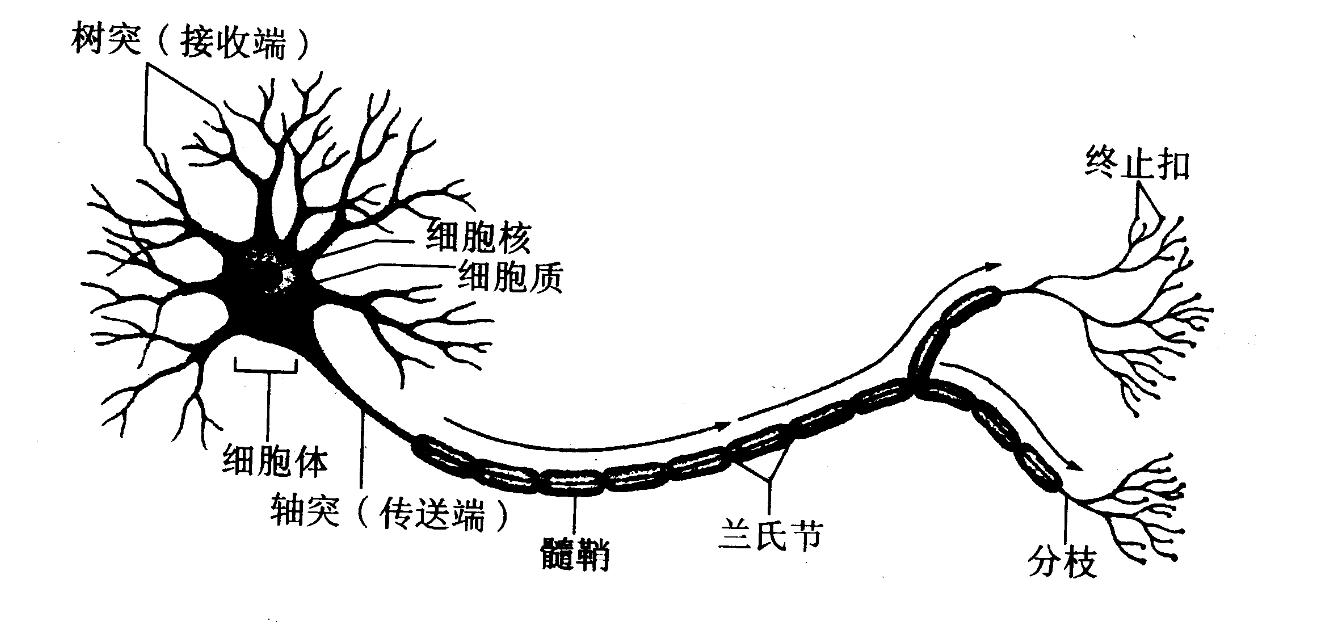
\includegraphics[height=6cm]{neuron}
  \caption{生物神经元的结构以及信息传递方式}
%  \label{fig:xfig1}
\end{figure}

%神经网络中的神经元可分为三个部分:输入信号、连接权重和激活函数。人脑皮层神经系统成为了人工神经网络出现的基础。人工神经网络的工作机制就是模仿生物神经元处理信息的机制,其中人工神经网络中的神经元相当于人脑神经系统中的神经元,通过激励和反馈,传递和处理信息。1943年,美国心理学家在总结了生物神经元基本特性的基础上,首先提出了神经元的数学模型,该模型很好地抽象了生物神经元的本质,并且忽略了复杂的生理学细节。该模型的提出,大大促进了人工神经网络的相关研究工作。


\subsection{人工神经网络概念}
人工神经网络就是由大量神经元组成多个网络层,将网络层相互连接组成的网络结构,其中多层前馈感知器就是其中最具代表性的一个模型。多层前馈感知网络是由2-3层网络层组成,对于相邻网络层中,上层网络层的神经元输出作为下层网络层的输入,同层内的神经元间相互独立没有连接。该网络结构保证输入信号从输入端开始传入,在网络中信号只是单方向地在网络处理与传递。

\begin{figure}[H] % use float package if you want it here
  \centering
  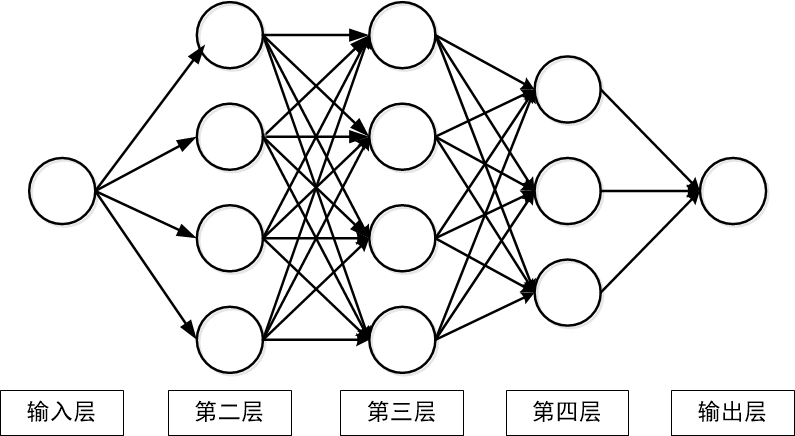
\includegraphics[height=6cm]{forward}
  \caption{人工神经网络的前馈网络}
  \label{fig:system}
\end{figure}


根据功能,根据多层前馈神经网络的信息处理方式和结构位置,其可以分为三个部分:第一部分是输入层,位于网络结构的起始段,作为输入信号进入网络结构的通道;第二部分是隐藏层,主要指在网络结构中由多个网络层的总称,其功能是实现数据的处理与计算功能;第三层是输出层,位于网络结构的终止端,用来输出前馈网络的计算结果。


神经元单元是神经网络系统中最重要的基础,一个神经元可简要地分为为三个部分:输入信号,连接权重和激活函数。神经元的工作机制可归纳为:处于抑制状态下的神经元,其树突接收到来自其他神经元所传递的兴奋激励信息,该激励信息可以由多个神经元所传递的信息组成;如果该激励信息超过某个限定值,那么接收信息的神经元则会由抑制状态转换为兴奋状态。


\begin{figure}[H] % use float package if you want it here
  \centering
  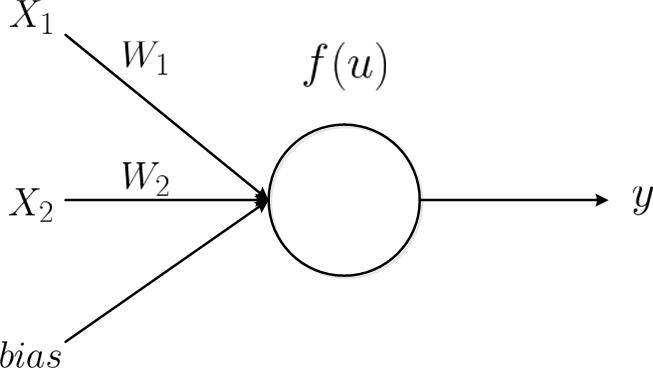
\includegraphics[height=4cm]{activation}
  \caption{人工神经网络中的神经元中信息传递过程}
  \label{fig:neuron}
\end{figure}


神经元的模型如图~\ref{fig:neuron}所示,该神经单元将接受的信息$X_1$,$X_2$,$\dots$,$X_n$,作为基础输入,这些输入就是原始输入信息或者上一个神经元所传递过来的信息;连接线条的数值$W_1$,$W_2$,$\dots$,$W_n$表示神经元之间具体的连接系数,即连接权值,表示轴突之间神经元的连接强度,通过点积的形式合输入相互结合,再加上一个偏置项对输入进行调整,通过激活函数$f(x)$进行判断,得到该神经单元最后的输出结果。激活函数通常是sigmoid函数和双曲正切函数,但是随着神经网络结构的不断地改进与复杂化,越来越多种形式的激活函数被应用到神经网络中。

图~\ref{fig:neuron}中的神经元模型具体的数据传递与激励计算过程可以表现为下列形式:
\begin{equation}
y=f(W_1 X_1 + W_2 X_2 + b)
\end{equation}

%人工神经网络系统就是大量的神经元互相连接而形成的复杂网络系统,即通过将多个网络层组装在一起形成一个复杂的网络系统,而相邻网络层之间就是用网络层内的神经元实现连接,多个神经元以权值表示连接强度实现连接,一个神经元的输出就是下一层的另一个神经元的输入,通过多个网络层的信息传递最终传输到输出层,得到网络的预测结果。
人工神经网络系统就是大量的神经元互相连接而形成的复杂网络系统,即通过将多个网络层组装在一起形成一个复杂的网络系统。根据单个神经元的数据处理过程,即可推导出在含有多个神经元的人工神经系统中,信息的具体传递方式。在如图~\ref{fig:system}的人工神经网络中,不同层神经元的信息传播可以表达为以下形式:
\begin{equation}
u_{j}^{(l)} = \sum_{i=1}^{n} W_{ij}^{(l-1)} X_{i}^{(l-1)} + b_{j}^{(l-1)}
\end{equation}
\begin{equation}
X_{j}^{(l)}=f(u_{j}^{(l)})
\end{equation}
其中,$W_{ij}^{(l-1)}$表示第$l-1$层中的第$i$个神经元输出对应第$l$层中的第$j$个神经元输入对应的连接权值。$X_i^{(l-1)}$表示第$l-1$层中的第$i$个神经元的输出,作为第$l$层的多个输入之一,$u_{j}^{(l)}$表示从$l-1$层的输出和对应权值的点积以及偏置项的加权和,作为$l$层第$j$个神经元的输入值。$f(x)$表示该神经元的激活函数。$X_{j}^{(l)}$表示$l$层的第$j$个神经元的输出,即传递到$l+1$层的多个输入之一。

输入信号在神经网络中经过网络隐含层的处理与传递后,逐层传播,最后在输出层得到神经网络的输出预测值。随后将预测值与实际值进行比较,设置损失函数,表示网络的性能,即对样本数据的拟合与表达能力。损失函数越小,则表示网络的预测值越符合真实情况,网络的性能越好;否则相反。根据具体要求不同,网络所采用的损失函数也是不一样的,比较常见的损失函数有:平方损失函数、指数损失函数、Hinge损失函数和log对数损失函数等。

\begin{equation}
h_{W,b}(X)=f(u^{(l)})
\end{equation}
\begin{equation}
E=\frac{1}{2m}\sum_{i=1}^{m}[h_{W,b}(X)_{i}-y_{i}]^{2}
\end{equation}
上述公式中的$h_{W,b}(X)$表示了网络的输出值,$y_{i}$表示了样本数据对应的实际值。假设这里的网络中使用了平方损失函数,则就要将预测值与实际值之间的差值进行平方处理,形式就如上述的损失计算公式。

如果根据图~\ref{fig:system}所示的话,而该网络的输出值和损失函数可表示为如下形式:
\begin{equation}
h_{W,b}(X)=f(u^{(5)})
\end{equation}
\begin{equation}
E=\frac{1}{2}(h_{W,b}(X)-y))^{2}
\end{equation}

\subsection{反向传播算法}

反向传播算法(Back-Propagation),也叫做误差反向传播或BP算法,常与最优化求解(如梯度下降法)相结合使用的,用来训练人工神经网络的经典方法。如果在训练过程中,使用了反向传播算法的网络,则也可称之为BP网络。BP算法的提出,使其成为了在监督学习的方式下训练多层前馈神经网络的典型且有效的方法,而且使神经网络开始具有广泛的应用潜力,也是目前最广为人知的人工神经网络模型之一。

BP算法是基于误差修正学习规则,使用梯度下降算法来最小化预测输出值与样本数据真实值之间的差值所构成的损失函数。BP算法实际上就是利用输出层的误差,来推导计算输出层上一层网络层神经元对应的误差数值,再利用所得到的误差数值继续推导计算更前层网络层相对应的误差值,以此类推,根据输出端预测误差逐级计算得到各层网络层的误差值,并且将这些梯度误差值沿着与输入信号传送相反的方向传递,则称之为反向传播算法。

BP网络主要是基于误差反向传播的多层前馈网络,但是早期的多层前馈神经网络只有信息的前向传播,BP网络提升了前馈网络的性能。与之前所使用的多层前馈网络相同,BP网络同样是由三个部分组成:输入层、隐含层和输出层;网络层之间的神经单元采用全连接方式传递数据,同层神经元之间独立无相互连接,这些特性都与之前提出的前馈神经网络相同。在BP网络结构中,输入层和输出层的神经元个数是由实际情况决定的,可以通过设置网络隐含层的层数以及每层中神经元节点的数目提升网络性能。

但是与之前所提出的前馈神经网络不同,BP网络最关键的地方通过误差信息的反向传播,调整网络中的权值,其学习的过程可以归纳为两部分:(1)输入信息的正向传播。在输入层传进数据信息作为输入信号,经过隐含层的数据处理和计算,最后在输出层输出预测结果值;信号在网络传递的过程中,网络中的连接权值是恒定不变的,每一层神经元的状态只会对下一层神经元的状态产生作用,对其他网络层没有影响。而网络中的每一层的权值是在反向传播过程中,通过对实际结果与预测结果的误差,对网络中的各层的权值进行调整,使网络最终的预测值更靠近实际结果。(2)误差信息反向传播:网络输出的预测结果值与样本数据的真实值比较的差值,即为误差信号。误差信息由输出端开始逐层沿着与输出信号传递相反方向进行传播,直到网络的输入端。输入信号的传递为前向传播,逐层朝正向方向递进传播;而误差信号的传递是沿相反方向实现传递,则为反向传播。在误差信号的反向传播过程中,网络的权值根据误差值的大小,不断改进网络的连接权值,通过迭代式地对连接权值进行修改,提升网络性能,使网络的输出预测值更接近实际样本的真实值。

\begin{figure}[H] % use float package if you want it here
  \centering
  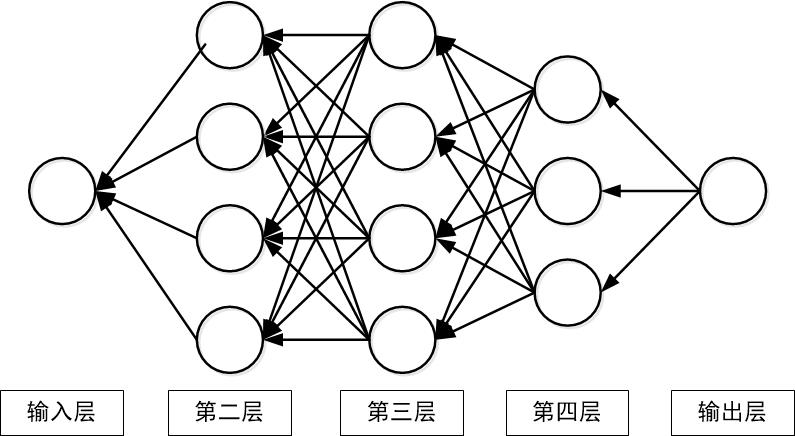
\includegraphics[height=6cm]{bp}
  \caption{人工神经网络中的误差反向传递的过程}
  \label{fig:bp}
\end{figure}

如图~\ref{fig:bp}中所示的在神经网络误差信息反向传播,该网络最终的输出可以表达为:
\begin{equation}
h_{W,b}(X)=f(u^{(5)})
\end{equation}

在这个网络中,损失函数通过log对数的形式表达,该方式如下:
\begin{equation}
J(W,b)=E=-\frac{1}{m}[\sum_{i=1}^{m} y_{i} log(h_{W,b}(X)_{i}) +
		(1-y_{i})log(1-h_{W,b}(X)_{i})]
\end{equation}
其中$h_{W,b}(X)_{i}$表示神经网络输出层的第$i$个输出单元的输出值,$y_{i}$表示样本数据中对应的第$i$个实际值,$J(W,b)$是根据网络输出层误差所计算的损失函数$E$的另一种形式。

由于反向传播算法传播的主要是每一层的相对误差信息,并且通过比较图~\ref{fig:system}和图~\ref{fig:bp}可以看出,误差信息的传播方向和输入信息的传播方向恰恰相反,在这里输入端的误差作为输入信号,在网络中进行传播。因此,首先需要计算输入层的误差,其表达形式如下:
\begin{equation}
\delta_{j}^{(5)}=h_{W,b}(X)_{j}-y_{j}
\end{equation}
在网络的反向传播中,都使用$\delta$表示所传递的误差值,则$\delta_{i}^{(5)}$表示第$5$层输出层中第$i$个神经元的误差值。

而对于之前的隐含层的误差计算,由于激励函数的存在,因此误差在经过激励函数时,需要对激励函数进行求导计算,因此,误差信息在隐含层的表示如下:
\begin{equation}
\delta_{i}^{(l-1)}=(\sum_{j=1}^{m} W_{ji}^{(l-1)} \delta_{j}^{(l)}) f'(u_{i}^{(l-1)})
\end{equation}

其中$\delta_{i}^{(l-1)}$表示$l-1$层中第$i$个神经元所计算的误差值,$W_{ji}^{(l)}$是第$l$层的第$i$个神经元对应第$l-1$层的第$j$个神经元的连接权值,为前向传播所对应的$W_{ij}^{(l)}$的转置形式,$\delta_{j}^{(l)}$表示$l$层中第$j$个神经元所计算得到的误差值。$f'(u_{j}^{(l-1)})$表示对$l-1$层的激励函数求导所得到的结果。

BP算法主要是根据梯度下降的方向,对问题进行求解,得到全局最小值作为最优解。在神经网络中,需要对网络层之间的连接权值$W_{ij}^{(l)}$和$b^{l}$进行更新,因此需要通过对损失损失函数用权值求偏导,求解最小梯度最小方向。
\begin{align}
\frac{\partial J(W,b)}{\partial W_{ij}^{(l)}} & = {\frac{\partial J(W,b)}{\partial u_{i}^{(l+1)}}} {\frac{\partial u_{i}^{(l+1)}}{\partial W_{ij}^{(l)}}}  \\
					    & =  X_{j}^{(l)} \delta_{i}^{(l+1)} \\
\frac{\partial J(W,b)}{\partial b_{i}^{(l)}} & = \frac{\partial J(W,b)}{\partial u_{i}^{(l+1)}} {\frac{\partial u_{i}^{(l+1)}}{\partial b_{i}^{(l)}}} \\
					    & = \delta_{i}^{(l+1)}
\end{align}

由以上公式,可以得到网络中每层对应的权值和偏置项的梯度方向,根据梯度下降法,则可以对权值$W_{ij}^{(l)}$和偏置项$b_{i}^{(l)}$进行更新:
\begin{align}
W_{ij}^{(l)} & = W_{ij}^{(l)} - \alpha \frac{\partial J(W,b)}{\partial W_{ij}^{(l)}}  \\
	     & = W_{ij}^{(l)} - \alpha X_{j}^{(l)} \delta_{i}^{(l+1)} \\
b_{i}^{(l)} & = b_{i}^{(l)} - \alpha \frac{\partial J(W,b)}{\partial b_{i}^{(l)}} \\
	    & = b_{i}^{(l)} - \alpha \delta_{i}^{(l+1)}
\end{align}
其中,$\alpha$表示网络初始设置的学习率。学习率为较大的值,可以使网络更快收敛,但是也可能造成网络得到局部最优解,甚至训练到一定程度后造成无法收敛的情况,因此学习率的设置也是非常重要的。

以上的计算实现了反向传播算法一次迭代的过程,但是在反向传播中需要实现多次迭代得到最优解,这里用$\bigtriangledown_{W^(l)} J(W,b)$表示$J(W,b)$对$W^{(l)}$的偏导,用$\bigtriangledown_{b^(l)} J(W,b)$表示$J(W,b)$对$b^{(l)}$的偏导。则反向传播算法的具体步骤可以表示为:
\begin{enumerate}
\item 初始化:对网络中所有层的权值$W_{ij}^{(l)}$和偏置项$b^(l)$进行初始化。
\item 进行前向传播,在网络计算输出值,以及损失函数值$J(W,b)$。
\item 进行反向传播,计算梯度$\bigtriangledown_{W^(l)} J(W,b)$和$\bigtriangledown_{b^(l)} J(W,b)$。
\item 更新各层的权值$W^{(l)}$和偏置项$b^{(l)}$,更新后逐步减小损失函数$J(W,b)$。
\item 判断是否达到迭代次数,如果达到次数,则进行下一步;如果没有达到次数,则返回第二步。
\item 根据网络输出,得到最终结果。
\end{enumerate}


%%%%%%%%%%%%%%%%%%%%%%%%%%%%%%%%%%%%%%%%%%%%%%%%%%%%%%%%%%%%%%%%%%%%%%%%%%%%%%%
\section{卷积神经网络}

\subsection{卷积神经网络发展历程}
卷积神经网络最初是受到生物神经学信息处理原理和机制的启发,成为人工神经网络众多网络模型中,流传最广、最常使用的网络之一。相对于普通特征提取方法而言,更强的适用性、特征提取能力、学习能力强和训练参数少是卷积神经网络最主要的特点。另外,卷积神经网络的泛化能力强等优点,使其成为图像识别相关领域非常重要的研究热点。

1962年,通过研究猫观察事物时,其神经的视觉皮层细胞的活跃情况,Hubel和Wiesel提出了感受野概念\cite{hubel1968receptive}。在人类的视觉神经系统中,人脑的输入神经信号是由眼睛上的视网膜光感受器接受光和场景信息所转换而成的。当感受器受刺激兴奋时,感受器官中的神经元会将外界的视觉信息以刺激信号的形式传递人脑更高级的神经细胞中,其中神经元用来对视觉信息产生刺激信号的区域就叫做神经元的感受野。

随后,感知机概念的提出是由Fukushima在20世纪80年代提出的\cite{fukushima1980neocognitron},其可以被认为是深度学习的起源,也可以视为卷积神经网络最初的表示形式,同时也是感受野相关概念首次实际应用于人工神经网络领域的。感知机与卷积神经网络不同的地方在于它没有使不同位置的神经元共享一个训练得到的权值;但是,感知机将所接收的视觉信息分解成多个较小模块化形式的低层次子特征,然后在这些低层次字特征通过多层次的特征平面化计算与处理,在区域平面化理的基础上,使用较少的计算量和参数量就能实现对输入数据的训练与传递,实现相应的识别。感知机是一个典型的多层神经网络模型,其中隐含层中的局部区域信息与局部感受野激发后生成了下一层的响应值。这种局部区域感受野的信息处理机制,可以避免信息处理过程中区域位置、大小和尺度的影响。另外,感知机采用的无监督学习也是卷积神经网络早期研究中占据主导地位的训练方式。 

1989年,LeCun在神经网络中的反向传播加入了一些限制,用来增强网络的学习能力,提高网络最终的预测能力\cite{lecun1998gradient}。他在训练 LeNet-5 网络的过程中使用了基于梯度下降方向传播算法,保证网络能够有监督学习与训练。手写数字图像在LeNet-5中多个卷积层、下采样层和全连接层的训练与作用下,图像转换为大量特征映射图,这些特征映射图就包含了高层次、抽象的辨别特征。卷积层中卷积核的作用相当于感知机中的区域感受野,通过卷积核的卷积处理,将图像中各个区域的局部信息提取为更具体、更有效、维度更小的特征信息。1998年,在手写数字体数据的识别中,使用深度学习技术的 LeNet-5 网络所取得的准确率超过了之前特征提取等方法的结果,而如今所流行的卷积神经网络模型都是沿用 LeNet-5 的卷积层、池化层和全连接层结构为模板而设计的。 

随后在2012年,卷积神经网络被Krizhevsky\cite{krizhevsky2012imagenet}等人应用在当年ImageNet的ILSVRC比赛,他们提出了名为AlexNet的卷积网络模型,并且赢得了比赛中图像分类和物体检测的双项第一名,在图像分类中领先第二名大约11\%的准确率,以极大优势获胜,这也是卷积神经网络在大规模自然图像数据中第一次的实际应用,实现了卷积神经网络性能的进一步提高,为深度学习在如今生活方方面面的应用拉开序幕。随后,不断有新的卷积神经网络模型被提出,比如牛津的VGGNet\cite{simonyan2014very},谷歌的GoogLeNet\cite{szegedy2015going},微软的ResNet\cite{he2015deep}等,这些网络模型不仅在ImageNet数据集上刷新着识别率记录,并且在其他许多数据集上也取得了最优异的结果,因此卷积神经网络在当前图像识别相关领域起着非常重要的作用。

由于基于卷积神经网络的深度学习结构具有非常强大的学习与表达能力,因此卷积神经网络不仅被应用在图像识别领域,而且也在视频分析和自然语言处理等方面具有很大的应用潜力,取得了非常好的成果。

%%%%%%%%%%%%%%%%%%%%%%%%%%%%%%%%%%%%%%%%%%%%%%%%%%%%%%%%%%%%%%%%%%%%%%%%%%%%%%%%%%%%%
\subsection{卷积神经网络原理和组成}

卷积神经网络最关键的部分为卷积核,卷积核与输入图像或者中间层的特征映射的不同小区域相连,通过卷积核的卷积处理,将图像信息具体化和转换,获取高层次特征信息。典型的卷积神经网络是由3种不同的神经层组成:卷积层,池化层和全连接层。传统的卷积神经网络是将卷积层和池化层进行组合连接的,以此来减少计算时间、逐步构建和提取更深层次的空间不变性。随后通过全连接层的特征转换,即可得到网络最终的输出。下面将主要介绍这个些结构单元的作用:

\begin{enumerate}
\item 卷积层

卷积层作为典型的深度神经网络,卷积神经网络中卷积层的每一个神经元是由前向传输层的局部感知域和所学习到的卷积核权值作为输入所组成的。在同一个特征映射图的神经元共享同样的卷积核,但是这个被共享的卷积核是用不同的输入感知域所得到的。在同一个卷积层中,由不同的特征映射所得到的卷积核是不同的。经过研究,卷积核的大小和数量表示了网络的宽度,网络宽度会对网络的性能造成影响。

实际上,在卷积层中,信息的前向传播主要是由上一层的特征映射和该层中可学习参数的卷积核进行卷积计算,再加上卷积层的偏置项的调整,经过激活函数进行计算处理的,就会得到该层每个卷积核所对应的输出特征映射。卷积层的卷积计算可以表达为以下公式:
\begin{equation}
X_{j}^{(l)} = f(\sum_{i} X_{i}^{(l-1)}  K_{ij}^{(l)} + b_{j}^{(l)})
\end{equation}
$X_{j}^{(l)}$表示第$l$层的卷积层的第$j$个输出特征映射;$X_{i}^{(l-1)}$表示第$l-1$层的第$i$个输出特征映射,即第$l$层的卷积层的输入;$K_{ij}^{(l)}$表示第$l$层中处理第$i$个输入特征映射到第$j$个输出特征映射所对于那个的卷积核;$b_{j}^{(l)}$是在第$l$层的第$j$个特征映射所对应的偏置项。在第$l$个卷积层的不同输出特征映射尽管是由相同的输入特征映射得到的,但是不同的输出特征映射所对应的卷积核是不同的。

\begin{figure}[H] % use float package if you want it here
  \centering
  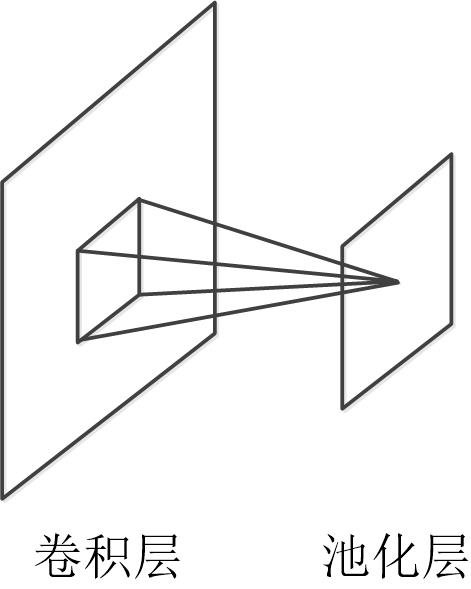
\includegraphics[height=5cm]{convolution}
  \caption{卷积神经网络中卷积层的信息处理}
\end{figure}


\item 池化层 

池化层是非线性下采样的一种形式,它的功能是不断减少表示特征的特征映射图的空间尺寸,用来达到减少参数数量和降低网络计算量的目的,另外也能实现控制过拟合的问题。而且,它也提供了平移不变性。池化层只是改变了输入映射图的尺寸,但是不改变输入映射的数量。平均池化和最大值池化是池化层比较常用的操作,其中最大值池化是最常用的操作,并且也应用在后续的实验当中。
\begin{equation}
X_{j}^{(l)} = f( \beta_{j}^{(l)} down(X_{j}^{(l-1)}) + b_{j}^{(l)})
\end{equation}			
其中$X_{j}^{(l)}$表示第$l$层的池化层的第$j$个输出特征映射;$\beta$是常量,用来控制池化层对数据的调整;$down(\cdot)$表示下采样处理,形式可能就是最大池化或者平均池化;$b_{j}^{(l)}$表示第$l$层的池化层中对第$j$个输出特征映射偏置的调整。因为池化层不改变特征映射数量,因此在这里经过池化处理,特征映射个数仍保持不变。

\begin{figure}[H] % use float package if you want it here
  \centering
  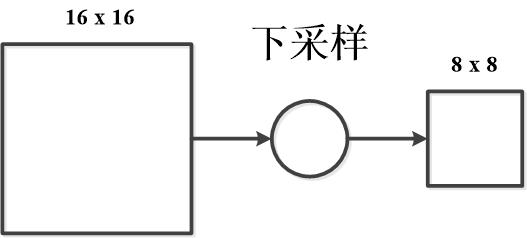
\includegraphics[height=3cm]{pooling}
  \caption{卷积神经网络中池化层的信息处理}
\end{figure}

\item 全连接层

全连接层的表示方式,就如常规的神经网络一样,全连接层中的神经元以全连接的形式进行数据的计算和信息的传递。因此,全连接层的激活函数可以通过矩阵乘法与偏差值计算来表示:
\begin{equation}
X_{j}^{(l)}=f(u_{j}^{(l)})=f(\sum_{i=1}^{m} W_{ij}^{l-1} X_{i}^{(l-1)} + b_{j}^{(l-1)})
\end{equation}
$X_{j}^{(l)}$是第$l$层为全连接层的第$j$个神经元的输出值;$W_{ij}^{l}$是第$l-1$层的第$i$个神经元到第$l$层的第$j$个神经元的连接权值;$X_{i}^{(l-1)}$是第$(l-1)$层中第$i$个神经元的输出值,$b_{j}^{(l-1)}$表示第$l-1$层对第$j$个输出特征映射的偏置,$f(x)$为激活函数。全连接层的计算方式与普通人工神经网络的传递方式基本相同,而且也是卷积神经网络中占据大量的参数和计算量的部分。

\end{enumerate}


%%%%%%%%%%%%%%%%%%%%%%%%%%%%%%%%%%%%%%%%%%%%%%%%%%%%%%%%%%%%%%%%%%%%%%%%%%%%%%%%%%%%%%%
\subsection{卷积神经网络的反向传播}

卷积神经网络的反向传播算法与普通人工神经网络的反向传播算法相同,也是将误差进行反向传播,同时根据梯度下降法,对网络中的参数进行调整与更新。卷积层、池化层和全连接层是卷积神经网络的基础部分,在卷积层和池化层中的信息处理和传递与普通前向传播方法不同,由于卷积层和池化层中传输的为特征映射,因此卷积神经网络的误差主要也是以特征映射的形式进行反向传播的,可称之为特征映射误差。对于全连接层,其前向传播和后向传播与普通神经网络相同,计算方式已在之前章节提到。所以接下来主要介绍卷积层和池化层的信息反向传播。 

\begin{enumerate}
\item 卷积层

假设目前第$l$层为卷积层,后面一层第$l+1$层为池化层,根据反向传播算法可知,为了要计算第$l$层的误差,我们需要知道$l+1$层的误差以及该层神经元所传递的输入加权和$u^{(l)}$。对于从卷积层到池化层的信息传递,实际上是卷积层一块像素组成的输出特征映射,变换为池化层的一个像素;因此,池化层中某点的误差,就对应了卷积层中某块像素对应的特征映射的误差值。为了保证有效计算出第$l$层卷积层中误差,将第$l+1$层池化层中的误差进行上采样处理,使其具有和卷积层的映射具有相同的尺寸,然后再将上采样的误差与$l$层的激活函数导数进行点乘即可。
\begin{equation}
\delta_{j}^{(l)} = \beta_{j}^{(l+1)} ( f'(u_{j}^{(l)}) * up(\delta_{j}^{(l+1)}))
\end{equation}
其中,$up(\cdot)$表示上采样处理,只是将输出的像素在水平方向和竖直方向拓展一定的倍速,形成一块像素区域,区域中每个像素值都相同;$\delta_{j}^{(l)}$表示第$l$层卷积层第$j$个特征映射对应的误差,$\beta_{j}^{(l+1)}$是第$l+1$层池化层中的常量,表示对误差进行相应的运算;$f'(u_{j}^{(l)})$表示激活函数的导数。

在计算出特征映射误差的前提下,通过对所有误差求和即可得到偏置项的梯度,其中$(u,v)$表示输出特征映射像素点的位置:
\begin{equation}
\frac{\partial E}{\partial b_{j}^{(l)}} = \sum_{u,v} (\delta_{j}^{(l)})_{uv}
\end{equation}

而对于网络层中卷积核的权值也可以用所得的误差计算得出:
\begin{align}
\frac{\partial E}{\partial K_{ij}^{(l)}} & = \sum_{u,v} (\delta_{j}^{(l)})_{uv} (p_{i}^{(l-1})_{uv} \\
					 & = rot180(conv2(X_{i}^{(l-1)}, rot180(\delta_{j}^{(l)})))
\end{align}
其中$(p_{i}^{(l-1})_{uv}$是$X_{i}^{(l-1)}$中与$K_{ij}^{(l)}$进行卷积计算的像素块,为了计算得到输出特征映射$X_{j}^{(l)}$中在位置$(u,v)$的像素;$rot180(\cdot)$表示对矩阵进行旋转180度处理;$conv2(\cdot)$表示卷积运算。

在求得卷积核偏导数和偏置项的偏导数后,即得到卷积核参数和偏置项的梯度方向,即可更具下列公式对卷积神经网络的参数进行更新:
\begin{align}
K_{ij}^{(l)} & = K_{ij}^{(l)} - \bigtriangledown_{K_{ij}^{(l)}} E \\
b_{j}^{(l)} & = b_{j}^{(l)} - \bigtriangledown_{b_{j}^{(l)}} E 
\end{align}
\item 池化层

假设目前第$l$层为池化层,后面一层第$l+1$层为卷积层,这种情况与之前的完全相反。但是同样,首先需要算出第$l+1$层的误差值。如果计算出了误差值后,则只需要对参数$b$进行更新即可。如果池化层后紧随的是全连接层,那么采样层的误差则可根据普通神经网络的反向传播算法进行计算。

一般情况下,如果池化层如果没有偏置项,则池化层不需要进行权值更新,但是仍然需要计算特征映射误差。当要计算卷积层中卷积核的梯度时,必须确定卷积层中输入特征映射中像素块所对应的输出特征映射的像素值。然而,在池化层必须确定特征映射误差的像素块对应下一层特征映射误差的像素值。则池化层的特征映射误差可以表示为:
\begin{equation}
\delta_{j}^{(l)}=f'(u_{j}^{(l)}) * conv2(\delta_{j}^{(l+1)}, rot180(K_{j}^{(l+1)})
\end{equation}
其中$\delta_{j}^{(l)}$表示第$l$层为池化层的第$j$个特征映射误差;$f'(u_{j}^{(l)})$表示激活函数的导数;同样,$rot180(\cdot)$表示对矩阵进行旋转180度处理;$conv2(\cdot)$表示卷积运算。
\begin{align}
\frac{\partial E}{\partial b_{j}^{(l)}} & = \sum_{u,v} (\delta_{j}^{(l)})_{uv} \\
b_{j}^{(l)} & = b_{j}^{(l)} - \bigtriangledown_{b_{j}^{(l)}} E 
\end{align}
对于池化层的偏置项求导与卷积层的偏置求导方法相同。同样,池化层的偏置项参数更新也与卷积层相同。

\end{enumerate}

%%%%%%%%%%%%%%%%%%%%%%%%%%%%%%%%%%%%%%%%%%%%%%%%%%%%%%%%%%%%%%%%%%%%%%%%%%%%%%%%%%%%%%%
\subsection{卷积神经网络模型}

\begin{enumerate}
\item LeNet-5\cite{lecun1998gradient}

LeNet-5是一个用来识别手写数字体图像的卷积神经网络,也是第一个可以实际应用于工业界的卷积神经网络,如今所提出的卷积网络模型都是参考了LeNet-5的模型所设计的。LeNet-5网络模型同样采用前向传播和后向传播的方法进行训练,但是由于每个网络层内部的权值共享,因此在保证了LeNet-5学习能力的前提下,大大减少了训练参数,加快了训练速度。LeNet-5网络模型不包括输入层,总共有7层网络层,每一层都包括可训练的权值参数,采用了交替连接的卷积层和下采样层对输入图像进行前向传导,并且最终通过全连接层输出概率分布的结构,LeNet-5网络模型如图~\ref{fig:lenet}所示。

\begin{figure}[H] % use float package if you want it here
  \centering
  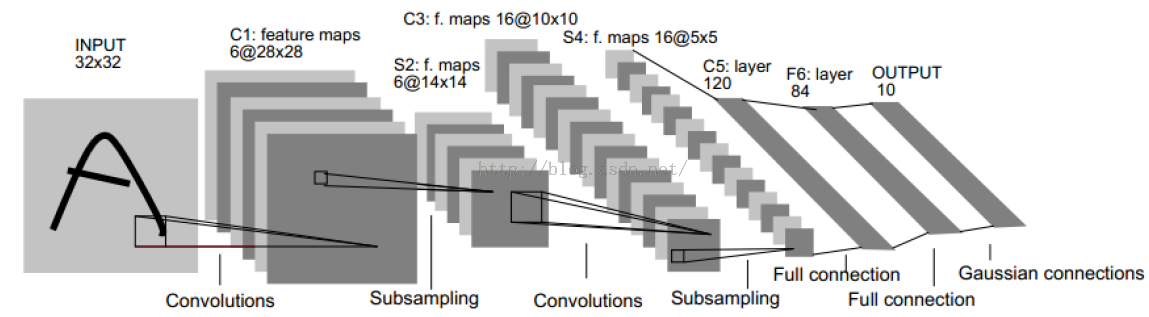
\includegraphics[height=3.5cm]{lenet}
  \caption{LeNet-5卷积神经网络模型}
  \label{fig:lenet}
\end{figure}


\item AlexNet\cite{krizhevsky2012imagenet}

在2012年的图像大规模视觉识别挑战赛 (ImageNet Large Scale Visual Recognition Challenge, ILSVRC)上,基于卷积神经网络的AlexNet横空出世,在图像分类和物体检测中都取得了双项冠军,在图像分类竞赛中相比于第二名在准确率上取得了高出11\%的优势,使得卷积神经网络的研究从此引起了学术界的高度关注,也开启了深度学习在各个领域应用的大门。AlexNet有5层卷积层,以及3层全连接层,约65万个神经元以及6000万个可训练参数,从网络规模上大大超越了LeNet-5。AlexNet使用了修正线性单元(Rectified Linear Units,ReLU)作为激活函数,取代了传统的sigmoid函数或tanh函数。而使用修正线性单元的网络训练速度将比使用tanh函数的网络快了将近六倍左右。局部响应归一化(Local Response Normalization,LRN)在训练过程中对所有输入信息进行归一化处理,保证邻近抑制,促进了训练速度。另外,深度网络经常会在训练过程中产生过拟合问题,造成网络性能下降,而基于dropout的技术,从一定程度上减轻了网络过拟合问题,提升了网络的准确率。另外,AlexNet还使用了多显卡进行网络的训练,与传统的处理器运算相比,显卡的逻辑运算功能大大强于处理器,在训练速度上提高了十多倍以上。AlexNet网络模型如图~\ref{fig:alexnet}所示。
%AlexNet满足了深度学习最基本的三个要求:大量的训练数据,合理的网络结构和强大的学习能力。

\begin{figure}[H] % use float package if you want it here
  \centering
  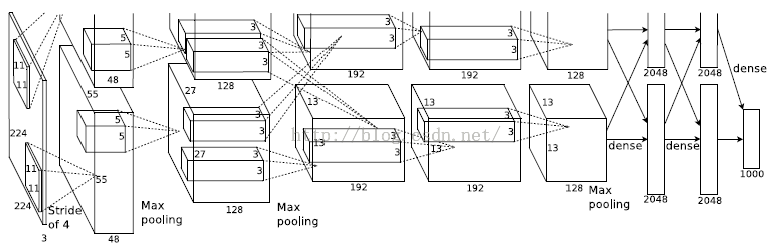
\includegraphics[height=4cm]{alexnet}
  \caption{AlexNet卷积神经网络模型}
  \label{fig:alexnet}
\end{figure}

\item GoogLeNet\cite{szegedy2015going}

Google公司在2014年的图像大规模视觉识别挑战赛 (ImageNet Large Scale Visual Recognition Challenge, ILSVRC)上,提出了GoogLeNet卷积神经网络模型。GooLeNet是一个具有22层网络层的深度卷积神经网络,这个模型最主要的特点就是提出了Inception单元,大幅度提高了网络计算资源的非线性能力。Inception是一个人工设计实现的非线性计算单元,在保持计算损耗不变的前提下,提升了网络的深度与宽度,以此来提高了网络的计算能力与非线性的表达能力。为了提高求解能力,GooLeNet还采用了Hebbian准则和多尺度处理方法来提高决策能力。GoogLeNet主要从两个方面提高网络模型的学习能力:网络的深度(网络层数)和网络的宽度(卷积核数量),但是相对产生的问题就是网络太深,梯度可能会消失,难以训练;参数太多,容易造成过拟合;以及网络计算复杂度太大,难以应用。为了解决以上问题,GoogLeNet从两个方面进行解决:(1)深度上,GoogLeNet为了避免梯度消失问题,在不同深度的位置增加了两个损失函数保证梯度顺利地回传;(2)宽度上,将多尺度的卷积核和池化处理组合成一个Inception单元结构,不仅可以减少网络参数,降低网络计算复杂度,而且很好地提升了网络的非线性表达能力。同时,Inception单元结构也是GoogLeNet最突出的特点,其具体结构如图~\ref{fig:inception}所示。

\begin{figure}[H] % use float package if you want it here
  \centering
  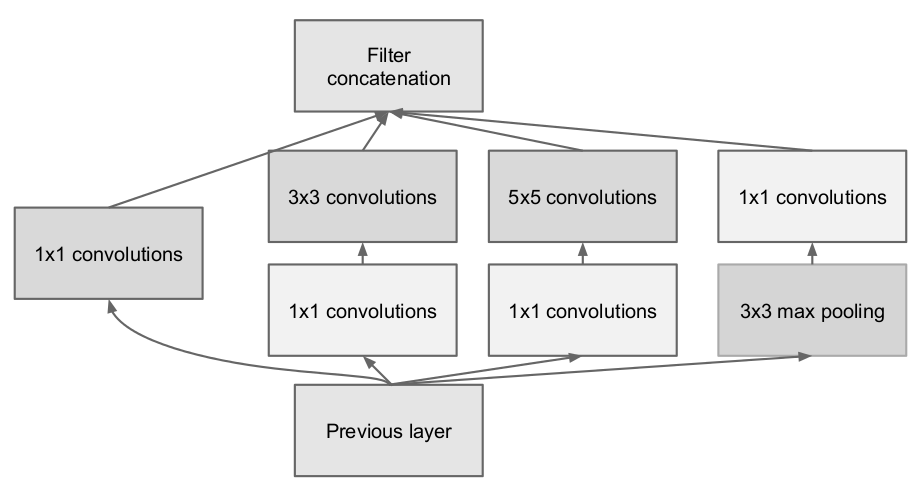
\includegraphics[height=4.5cm]{inception}
  \caption{GoogLeNet网络模型中的Inception单元结构}
  \label{fig:inception}
\end{figure}

\end{enumerate}



\section{本章总结}
本章主要介绍了深度学习的相关概念,人工神经网络中的生物神经基础、基本知识和反向传播算法,以及卷积神经网络的原理、机制和模型。深度学习是机器学习领域一个新的研究方向,以大量的样本数据为基础,在具有深层次的网络结构的条件下,通过庞大的计算量以及有效的训练方法使网络学习和表达数据中潜在的规律,实现网络对数据的拟合与预测。因此,人工神经网络是深度学习的基础,而人工神经网络是收到生物神经系统的启发而研究的,其目的在于模拟人脑中对于信息的处理方式来处理和分析大量的数据。人工神经网络具有前向传播和后向传播两种方式,其中后向传播算法是保证网络能够得到有效训练,更符合数据规律的关键。

卷积神经网络是深度学习中一个经典、应用最广泛的算法之一,目前已经在图像识别、视频分析、自然语言处理等各个领域取得了非常显著的成绩。卷积神经网络主要是由卷积层、池化层和全连接层组成,其从样本数据出发,隐式地从训练数据中学习规律;由于局部权值共享的特点,很大程度减少了需要训练参数数量,大大降低了网络复杂性,提取和转换平移、尺度和其他形式的扭曲不变形特征,具有非常好的效果。










\chapter{卷积神经网络各因素对图像分类的探究}

\section{数据集介绍}

传统的浮游生物调查主要是通过在一块区域内的水采样实现的,但是这种传统方法很难满足目前实际研究的需求,现在的浮游生物研究要求长时间持续性的观察和大规模快速实时的分析,因此目前越来越多的原位浮游生物图像采集系统正在处于开发与使用阶段,例如VPR(Video Plankton Record)\cite{davis2005three}以及SPC(Scripps Plankton Camera)\cite{benfield2007rapid}等设备。科学家们正在不断使用基于图像技术的设备来研究浮游生物的生物特性,通过这些系统或设备,可以很好地研究浮游生物的生态系统。因此,相关机构公开了越来越多的浮游生物图像相关的数据集。下面将介绍三个公开在网络上,使用较为频繁的的浮游生物灰度图像数据集:

\begin{enumerate}
\item ZooScan数据集\footnote{http://www.zooscan.obs-vlfr.fr}

在扫描仪器技术上的快速发展,使短时间内对大量的浮游生物个体进行高质量数字图像化的采集具有可行性和应用性。ZooScan是浮游动物图像扫描分析系统,适用于采集体型微小的浮游生物图像,并且能够快速分析获取图像中浮游生物在形态特征各方面的信息。在这个ZooScan采集到的数据集中,总共有13类浮游动物图像,被分为两个部分:训练集和测试集;其中,训练集图像为9460张图像,测试集为1300张图像。该数据集类别不多,且不同类别的图像数量分布较为平均,图像总数量适中。

\item Kaggle数据集\footnote{https://www.kaggle.com/c/datasciencebowl}

由于浮游生物对地球环境和生态系统的重要性得到越来越多人的关注,但是人工对浮游生物图像的识别与分析的可行性很差,而自动化图像识别分析系统在海洋环境与生态系统的监测中有更广的应用前景。因此,Kaggle组织了国家科学数据杯赛(National Data Science Bowl),要求参赛者对浮游生物图像采取有效的算法实现自动化的图像识别处理,实现浮游生物图像的自动识别与分析。俄勒冈州立大学(Oregon State University)的哈特菲尔德海洋科学中心(Hatfield Marine Science Center)提供了大量的浮游生物图像,有13个种类总共30,000张图像。但是在该数据集中,存在部分浮游生物类别中只有1-2张图像,而有的浮游生物类别图像可达到几千张,是一个非常不平衡的数据集。在这个数据集的基础上,所训练的网络以及分类准确率都不够合理。

\item WHOI-Plankton数据集\footnote{http://darchive.mblwhoilibrary.org/handle/1912/7341 }

伍兹霍尔海洋研究所(Woods Hole Oceanographic Institution)使用了IFCB(The Imaging Flow Cytobot)系统来采集浮游生物图像\cite{orenstein2015whoi}。该系统是一个原位实时系统,从2006年开始就持续性地对浮游生物进行成像处理。到目前为止,该系统已经生成了超过7亿张样本图像。伍兹霍尔海洋研究所发布了一个巨大规模的、基于视觉识别的浮游生物数据集:WHOI-Plankton。该数据集的主要功能就是用于浮游生物分类的相关研究,其包含了70类超过340万张浮游生物图像。这些图像是由IFCB在近8年不断收集到的浮游生物图像数据所组成的。实际上,官方所提供的数据集中,是包含了103类超过300万张浮游生物图像。虽然该数据集在种类丰富度和图像数量上都非常充足,然而这103类浮游生物的数据集中,浮游生物图像的分布是非常不平衡的,其中有一类超过了200百万张图像,有部分浮游生物类别有10万张图像,然而也有的类别图像甚至低于500张。因此通过这种不平衡的数据集训练得到的网络模型,其分类准确率同样是不够合理的。

\end{enumerate}

根据以上三个数据集的规模和特点,以及深度学习实现的要求,在这里本论文选择ZooScan数据集和WHOI-Plankton数据集进行实验。由于ZooScan数据集数量和图像较少,可用来验证卷积神经网络在浮游生物图像分类上的可行性,以及探究影响卷积神经网络在浮游生物图像分类准确率的各个因素;WHOI-Plankton数据集中具有较多的浮游生物图像,以及较多类别的浮游生物,可以用来验证本论文所提出的基于多特征卷积神经网络模型。

%%%%%%%%%%%%%%%%%%%%%%%%%%%%%%%%%%%%%%%%%%%%%%%%%%%%%%%%%%%%%%%%%%%%%%%%%%%%%%%%%%%%%%%%%%%%%
\section{探究网络参数对分类结果的影响}

首先,为了验证深度学习学浮游生物图像分类问题的可行性,考虑到ZooScan数据集的浮游生物种类和数量比较合适,因此将当前流行的卷积神经网络模型应用在ZooScan浮游生物数据集上,并且通过对网络中几个重要的参数进行修改设置,判断卷积神经网络在浮游生物图像数据集上的可行性,以及探讨在卷积神经网络的哪些因素在浮游生物图像数据上起着关键作用。本论文主要从以下四个方面进行实验:数据集图像数量、网络层数,卷积核的尺寸和数量,不同的修正线性单元作用。而对于结果而言,准确率、训练损失值、验证损失值、网络复杂度等都是衡量网络整体性能的重要指标。

在ImageNet数据集上取得了显著效果的卷积网络:AlexNet、CaffeNet、VGGNet和GoogLeNet都被应用在浮游生物数据集上,作为最基础的衡量指标。表一表示了这些网络模型在ZooScan数据集上的分类结果。造成这种结果可能的原因是尽管这些模型在自然场景分类任务下具有非常良好的能力,但是由于数据集本身在质量与数量上的限制,可能造成网络的学习和泛化能力降低,不能取得很好的效果。因此需要分析卷积神经网络的各个因素,对其进行改进提高准确率。这里的实验方法主要是采用自底向上的方法,通过对网络本身性质的探索,在实验的基础上研究出网络关键因素,根据这些因素提出适用于浮游生物数据集分类的卷积神经网络。本实验采用了AlexNet作为基础网络,因为AlexNet是第一个在ImageNet图像大规模视觉识别竞赛中取得优胜的深度学习网络模型,同时也是目前许多网络模型的雏形,可以很好地对其进行改造和设计。

\begin{table}[H]
%\small
\centering
\caption{在ZooScan数据集上,不同卷积神经模型所取得的结果}
\label{comparison}
\vspace{0.2em}
\begin{tabular}{|c|c|c|c|c|c|c|}
\hline 模型 & 准确率 & 训练损失值 & 验证损失值 & 结构 & 训练时间\\ 
\hline AlexNet  & 82.1\% & 0.4273 & 0.5385 & 5 Conv + 3 FC &  8 min\\
\hline CaffeNet & 81.6\% & 0.3422 & 0.5496 & 5 Conv + 3 FC &  8 min\\
\hline VGGNet  & 81.9\% & 0.3921 & 0.5175 & 13 Conv + 3 FC &  14 min\\
\hline GoogleNet & 82.1\% & 0.4618 & 0.5356 & -  & 15 min\\
\hline  
\end{tabular}
\end{table}


\subsection{数据增强}

数据量是深度学习最关键的因素之一,在大量数据的基础上,深度学习可以探索出数据内部所隐藏的最本质的规律,以及表达出数据中最具代表性的模式。然而,因为数据量的缺乏,就算学习能力强的神经网络,也无法探索与表示具有代表性的特征与模式,也就不能取得很好的结果。

由于ZooScan数据集中包含13类浮游生物总共9460张浮游生物图像,虽然对于普通机器学习的方法,这规模的数据集已经有了足够的图像,但是对于深度学习而言,所需要的数据量却仍然是不够的,最后造成的结果可能就是较低的分类准确率以及过拟合现象的发生。因此,必须采取有效的方法提升数据规模,同时这也是最有效的方法来解决训练过程中的过拟合问题,从本质上对深度学习的结果进行提升。

对于浮游生物图像而言,旋转不变性和平移不变性是非常重要的特性,因此这里主要采用了旋转和平移的方法来增加数据集的规模,并且再增加其它几种数据增强方法,使数据更加多样性:

\begin{enumerate}
\item 旋转:随机将图像旋转90度、180度、270度中的任一角度;
\item 平移:随机将图形向水平方向或垂直方向平移40个像素;
\item 缩放:随机将图像中的浮游生物放大或缩小1.2倍;
\item 镜像:随机将图像根据水平方向或者垂直方向进行翻转映射;
\item 斜切:随机将图像由正20度或者负20度的斜切变换;
\end{enumerate}

\begin{figure}[H]
\centering
\begin{minipage}[]{0.3\linewidth} 
      \centering 
      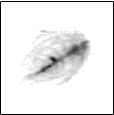
\includegraphics[height=2.5cm]{origin}
        \centerline{(a) 原始图像}\medskip
\end{minipage}
  \begin{minipage}[]{0.3\linewidth}
    \centering
    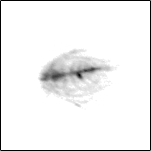
\includegraphics[height=2.5cm]{rotation.png}
      \centerline{(b) 旋转}\medskip
  \end{minipage}
  \begin{minipage}[]{0.3\linewidth}
    \centering
    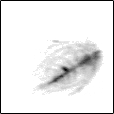
\includegraphics[height=2.5cm]{translation}
      \centerline{(c) 平移}\medskip
  \end{minipage}
\begin{minipage}[]{0.3\linewidth} 
      \centering 
      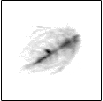
\includegraphics[height=2cm]{resize}
        \centerline{(d) 缩放}\medskip
\end{minipage}
  \begin{minipage}[]{0.3\linewidth}
    \centering
    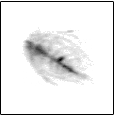
\includegraphics[height=2.5cm]{mirror}
      \centerline{(e) 镜像}\medskip
  \end{minipage}
  \begin{minipage}[]{0.3\linewidth}
    \centering
    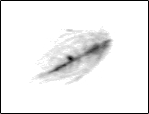
\includegraphics[height=2.2cm]{shearing}
      \centerline{(f) 斜切}\medskip
  \end{minipage}
  \caption{原始图像,以及使用不同数据增强方式得到的结果}
\label{fig:augmentation}
\end{figure}

表~\ref{tab:da}表示不同网络在经过数据增强的数据集上训练后,所得到的结果。从该表中可以看出,各个网络的分类准确率都有大幅度提升。尽管数据增强可以大量地增加图像数量,增加数据集的规模,在结果上,提升了网络的分类准确率;相应地也增加了网络的训练时间。然而在足够强大的硬件条件支持下,所增强的训练时间是能够省略的。

\begin{table}[H]
%\small
\centering
\caption{数据增强后,卷积神经网络在ZooScan数据集上的结果}
\label{tab:da}
\vspace{0.2em}
\begin{tabular}{|c|c|c|c|c|c|c|}
\hline 模型 & 准确率 & 训练损失值 & 验证损失值 & 结构 & 训练时间\\ 
\hline AlexNet  & 91.3\% & 0.0122 & 0.2263 & 5 Conv + 3 FC  & 28 min \\
\hline CaffeNet & 91.0\% & 0.0775 & 0.2435 & 5 Conv + 3 FC  & 28 min \\
\hline VGGNet  & 92.2\% & 0.0144 & 0.2011 & 13 Conv + 3 FC  & 54 min \\
\hline GoogleNet & 91.9\% & 0.0041 & 0.2454 & - &  57 min \\
\hline  
\end{tabular}
\end{table}



\subsection{网络深度}
近期相应的研究表明,网络的深度是主导其在数据集上性能的主要因素。网络深度也表示了深度学习的学习能力,越深的网络其学习能力越强。近些年在ImageNet数据集上取得优胜的深度学习网络模型都有非常深层次的网络结构。这也表示了网络的深度,即网络层数,是影响网络结果的最关键因素之一。因此,将网络从8层到16层的逐层拓展,可以得到不同的结果,通过观察与比较这些结果来推导出最后的结论。根据VGGNet网络的实验结论,将一些小卷积核的卷积层堆积起来,而不是使用一个大卷积核的卷积层,可以很好地增加网络的深度,而且还能降低网络参数、容量的消耗以及庞大的计算量。在这里,对于改进网络深度同样使用了卷积层堆积的方法。

\begin{table}[H]
%\small
\centering
\caption{在ZooScan数据集上,关于网络深度实验的五种网络结构形式}
\label{tab:config}
%\vspace{0.2em}
\begin{tabular}{|c|c|c|c|c|c|}
\hline 8层(AlexNet) & 9层 & 11层 & 13层 & 16层 \\ 
\hline \multicolumn{5}{|c|}{input (227 $\times$ 227 image crop)} \\
\hline \multirow{2}{*}{conv11-96} & \multirow{2}{*}{conv11-96} & \multirow{2}{*}{conv11-96} & \multirow{2}{*}{conv11-96} & conv7-96 \\
	& & & & conv7-96 \\
\hline \multicolumn{5}{|c|}{3$\times$3 maxpool} \\
\hline \multirow{2}{*}{conv5-256} & \multirow{2}{*}{conv5-256} & \multirow{2}{*}{conv5-256} & \multirow{2}{*}{conv5-256} & conv3-256 \\
	& & & & conv3-256 \\
\hline \multicolumn{5}{|c|}{3$\times$3 maxpool} \\
\hline conv3-384 &  conv3-384 & conv3-256 & conv3-256 & conv3-256 \\

	conv3-384 & conv3-384 & conv3-256 & conv3-256 & conv3-256  \\

	conv3-256 & & conv3-256 & & conv1-256 \\
	\cline{1-5} \multicolumn{5}{|c|}{3$\times$3 maxpool} \\
	\cline{1-5} &  conv3-384 & conv3-384 & conv3-384 & conv3-384 \\
	& conv3-384 & conv3-384 & conv3-384 & conv3-384  \\
	&  &  conv3-384 & conv1-384 & conv1-384 \\
	\cline{2-5} &  \multicolumn{4}{c|}{3$\times$3 maxpool} \\
	\cline{1-5} & & & conv3-384 & conv3-384 \\
	 & & & conv3-384 & conv3-384 \\
	& & & conv1-384 & conv1-384 \\
	\cline{4-5} & & & \multicolumn{2}{|c|}{3$\times$3 maxpool}\\

\hline \multicolumn{5}{|c|}{FC-4096}\\
\hline \multicolumn{5}{|c|}{FC-4096}\\
\hline \multicolumn{5}{|c|}{FC-13}\\
\hline \multicolumn{5}{|c|}{softmax layer} \\
\hline  
\end{tabular}
\end{table}

\begin{table}[H]
%\small
\centering
\caption{不同深度的网络在ZooScan数据上的结果}
\label{tab:dep}
\begin{tabular}{|c|c|c|c|c|c|c|c|}
\hline 模型 & 准确率 & 训练损失值 & 验证损失值 & 训练时间\\ 
\hline 8层 & 91.3\% & 0.0122 & 0.2263 & 28 min \\
\hline 9层 & 92.1\% & 0.0201 & 0.2255 & 29 min \\
\hline 11层 & 92.8\% & 0.0401 & 0.2722 & 34 min \\
\hline 13层 & 92.5\% & 0.0415 & 0.2612 & 44 min  \\
\hline 16层 & 92.3\% & 0.0455 & 0.2627 & 53 min  \\
\hline
\end{tabular}
\end{table}

表~\ref{tab:dep}表示在数据增强的前提下,不同深度的网络所得到的准确率结果。表~\ref{tab:config}表示不同网络深度下的网络结构设置,因为采用了卷积层堆积的方法,所以深度不是线性增长的。从表~\ref{tab:dep}中可以看出,在很高的分类准确率的前提下,网络深度的改进只能小幅度地提升网络性能。但是,随着网络的持续增加,在训练过程中将会消耗更多的时间,最后准确率反而还下降了。导致这种情况的发生,可能是由于梯度的消失或爆炸。


\subsection{网络宽度}
网络的宽度,即卷积层中卷积的大小和数量,是除了网络深度外,另一个影响网络学习能力的因素。在实验中,我们试过了许多不同尺寸的卷积核:13x13,11x11,7x7,甚至是三个5x5的堆积,来寻找合适大小的卷积核。而不同的卷积核数量256,384和512,也是我们考虑的另外一个方面。

表~\ref{tab:width}表示了不同卷积核设置下的图像分类结果。由于之前的结果表示11层卷积神经网络在浮游生物数据上能取得较好结果,因此对于网络宽度的修改,是基于11层网络为基础的。表~\ref{tab:width}第二列表示基础网络,随后各列表示不同宽度的网络配置,分别以A、B、C和D命名,各个网络的层数相同,只是卷积核的大小和数量不同。正常来说,11x11和7x7大小的卷积核在分类任务上可以取得很好的结果。但是在浮游生物图像分类上,将第一层卷积核设置为13x13,第二层卷积核设置为7x7,反而能取得很好的结果,相应也会带来计算量增大以及网络复杂度的增加。对此结果的推断是:由于图像只有浮游生物,因此大尺寸的卷积核能获取更多关于浮游生物有用的信息。相似地,更多数量的卷积核从更多维度来获取特征,因此384和512的卷积数量设置能够取得很好的结果。


\begin{table}[H]
%\small
\centering
\caption{不同大小和不同数量的卷积核的网络在ZooScan数据集上的结果}
\label{tab:width}
\begin{tabular}{|c|c|c|c|c|c|c|c|c|}
\hline  & 11层 & A & B & C & D \\ 
\hline \multirow{10}{*}{网络结构}& conv11-96 & conv13-96 & conv13-96 & conv13-96 & conv13-96 \\
	& & & & &  \\
	\cline{2-6} & conv5-256 & conv5-256 & conv7-256 & conv7-256 & conv7-256 \\
	& & & & & \\
	\cline{2-6} & conv3-256 & conv3-256 & conv3-256 & conv3-384 & conv3-512 \\
        & conv3-256 & conv3-256 & conv3-256 & conv3-384 & conv3-512 \\
        & conv3-256 & conv3-256 & conv3-256 & conv3-384 & conv3-512 \\
	& & & & & \\
	\cline{2-6} & conv3-384 & conv3-384 & conv3-384 & conv3-512 & conv3-512 \\
	& conv3-384 & conv3-384 & conv3-384 & conv3-512 & conv3-512 \\
	& conv3-384 & conv3-384 & conv3-384 & conv3-512 & conv3-512 \\
	& & & & & \\
\hline 准确率 & 92.8\% & 92.9\% & 93.1\% & 93.6\% & 93.6\% \\
\hline 训练时间 & 34 min & 35 min & 36 min & 39 min & 43 min \\
\hline 
\end{tabular}
\end{table}

\subsection{线性修正单元}
线性修正单元(Rectified Linear Units, ReLU)作为深度学习网络中的激活函数,起着非常重要的作用,保证了网络的正常训练。ReLU在训练过程中加速了收敛,代替了传统的sigmoid函数作用于当前的深度网络结构中。另外一些研究学者更关注修正单元的功能,提出了PReLU(Parametric ReLU)取代普通的ReLU模块,其可以逐步学习改进修正单元的参数。相比较于使用ReLU的卷积网络,使用PReLU的卷积网络在可忽略的额外计算量代价下,提升了最后的准确率。最终结果表示在表~\ref{tab:re}中,该结果是以表~\ref{tab:width}中11层网络结构的C配置为基础展开的。尽管PReLU在训练时间和准确率上只有轻微的影响,但是其仍然能够起到一定作用。

\begin{table}[H]
%\small
\centering
\caption{包含ReLU和PReLU的网络结构C在ZooScan数据集上的准确率}
\label{tab:re}
\begin{tabular}{|c|c|c|c|}
\hline 结构 & 准确率 & 训练时间\\
\hline C (ReLU) & 93.6\% & 39 min \\
\hline C (PReLU) & 93.7\% & 38 min \\
\hline 
\end{tabular}
\end{table}

通过以上多组实验,以及对实验结果的分析和讨论,可以得出:基于深度学习的卷积神经网络,可作为浮游生物图像分类问题的解决方案。影响浮游生物图像分类准确率的最主要因素是图像的数据增强;通过数据增强,可以提升数据集的多样性,保证网络充分训练;其次,卷积神经网络的深度与宽度同样是非常重要的因素,通过对深度和宽度的控制,虽然训练时间有所增加,但是仍然能提升图像的分类准确率。但是由于经过数据增强的提升,基础网络准确率已经达到很高的水准,因此通过对网络深度和宽度的修改,只能小幅度地提升结果;最后,对卷积神经网络中的激活函数和线性修正单元的改进,只是很小幅度地提升实验结果。因此,从上述实验结果,再次验证数据增强、网络深度和宽度是影响网络性能的最主要因素,对于浮游生物图像分类的结果同样适用。


%\begin{figure}[H] % use float package if you want it here
%  \centering
%  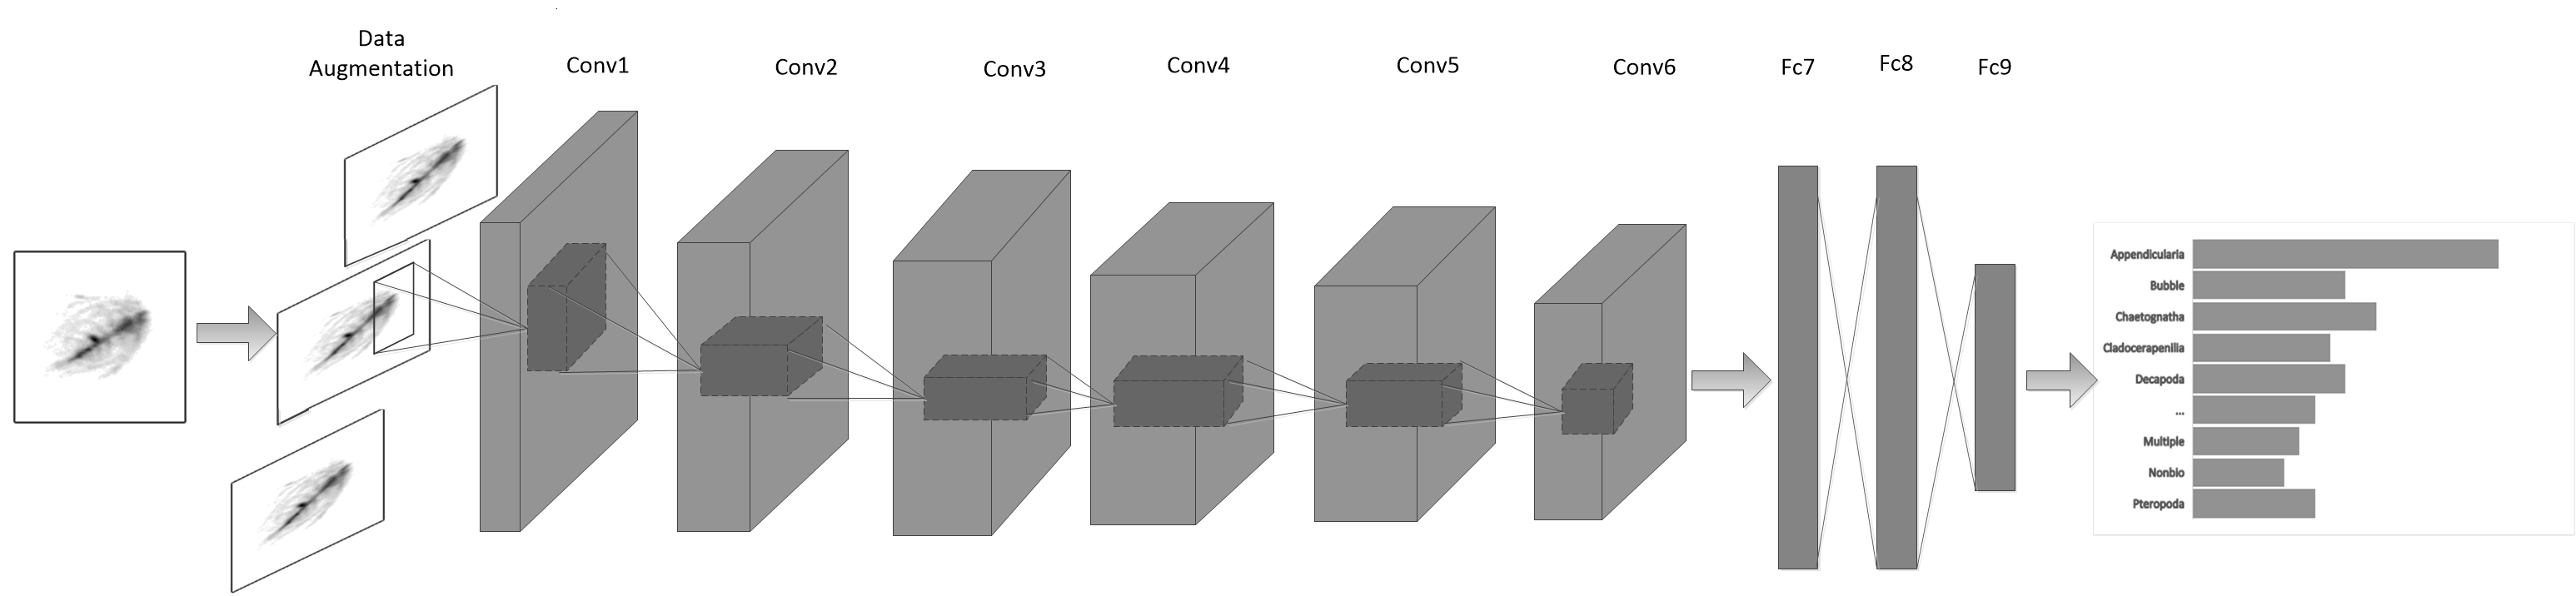
\includegraphics[height=3.8cm]{network}
%  \caption{对上述因素总结,所提出的基于浮游生物图像的单卷积神经网络模型}
%  \label{fig:xfig1}
%\end{figure}

%%%%%%%%%%%%%%%%%%%%%%%%%%%%%%%%%%%%%%%%%%%%%%%%%%%%%%%%%%%%%%%%%%%%%%%%%%%%%%%%%%%%%%%%%%%%%
\section{组合网络模型}

根据以上所得到的实验结果,AlexNet在网络的深度和宽度与其他卷积伸进网络模型相比,具有较大的改进空间和潜力,本章在AlexNet的基础上对应其进行改进和总结。根据之前网络深度和网络宽度的实验结果,对AlexNet进行修改,加上数据增强和改进线性修正单元,可总结得到应用于少量类别的浮游生物图像分类的卷积神经网络模型,称为ZooplanktoNet。由于该模型是基于13类浮游生物图像数据集进行训练的,因此只能应用于少量类别的浮游生物图像分类。图~\ref{fig:stack}表示该模型的具体结构。

\begin{figure}[H] % use float package if you want it here
  \centering
  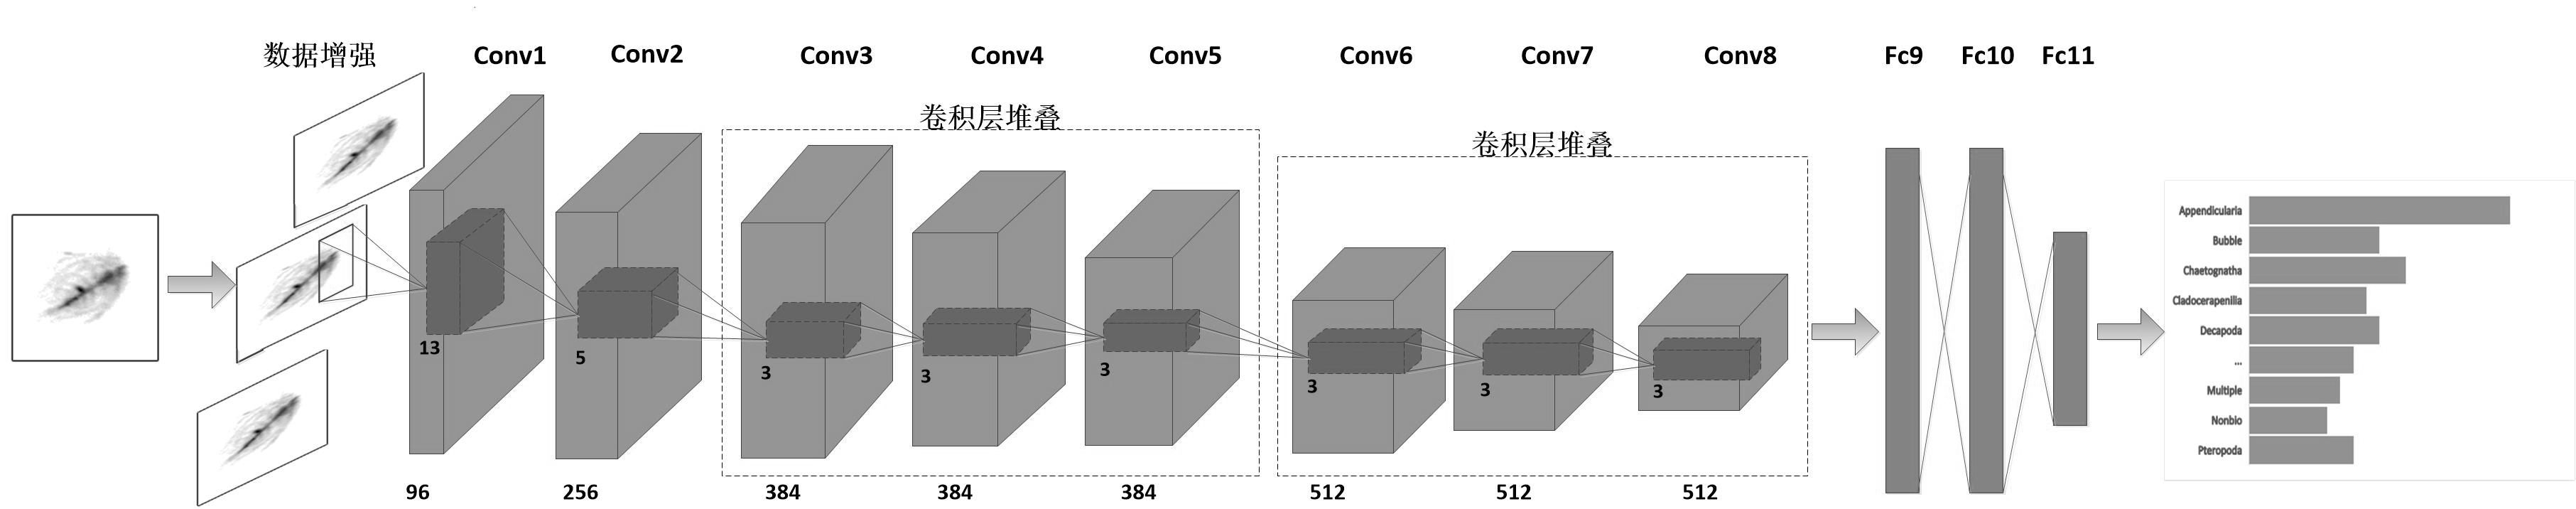
\includegraphics[height=3cm]{stack}
  \caption{应用于少量类别的浮游生物图像分类的卷积神经网络模型ZooplanktoNet}
  \label{fig:stack}
\end{figure}

首先,浮游生物图像数据集使用数据增强方法,扩大训练数据的规模;随后,训练数据经过8层卷积层和3层全连接层组成的卷积神经网络模型(其中,卷积层的卷积核大小和数量,随层数的增加,相应地减少和增大;且相邻的三个卷积层组成卷积层堆叠);最后,末尾的全连接层输出网络预测结果。表~\ref{tab:re}中的第二行实验数据,就是ZooplanktoNet在数据集上的分类结果。

通过以上实验证明,卷积神经网络模型ZooplanktoNet针对13类浮游生物图像,其准确率超过ZooScan扫描仪所能达到的最高准确率,能够有效解决少量类别的浮游生物图像分类问题。

%%%%%%%%%%%%%%%%%%%%%%%%%%%%%%%%%%%%%%%%%%%%%%%%%%%%%%%%%%%%%%%%%%%%%%%%%%%%%%%%%%%%%%%
\section{本章总结}

本章节主要介绍了浮游生物相关的数据集、在浮游生物图像分类中卷积神经网络性能影响因素的探究、以及提出了应用于浮游生物图像分类的卷积神经网络模型。根据所设置的多组实验的结果进行分析,证明数据增强、网络深度和宽度同样是影响卷积神经网络对浮游生物图像分类结果的最主要因素。另外,本章还将对这些结果进行总结,启发性地提出了一个应用于少量类别的浮游生物图像分类的卷积神经网络模型,在保证准确率和训练条件的前提下,能够有效实现图像的分类。













\chapter{多特征卷积神经网络的图像分类方法}


\section{浮游生物图像特点}
自然图像分类主要是将图像中不同物种或不同类别的物体进行相应的归属分类,不同类别或不同类别的物体之间在外观形态上具有较大的差异,因此可根据其外观上形态特点的不同进行区分判断。但是自然图像分类的难点在于物种和种类的多样性,一般的自然图像分类中的种类数目可能在10-100类之间,甚至会有1000类的情况,这为自然图像分类带来巨大难度。在传统的自然图像分类中,通常是对图像提取特定的特征,根据所提取的特征进行相应分类器的训练,使用训练好的分类器对图像进行分类。而细粒度图像分类是在相同基本类别或物种下,对其繁多的子类别进行区分。由于细粒度图像分类属于相同大类的分类,所以各子类别之间的差异很小,这些细微的差异很容易被形状、背景等变化因素影响,导致细粒度图像分类相对困难。因此,细粒度图像分类要求更关注某些具体的细节信息差异,设计更有效的算法实现高准确率分类。对于细粒度图像分类,通常是对某些局部的细节特征信息进行处理,根据这些细微差异进行判断。

浮游生物种群数量庞大,在这种数量级的情况下,不同种类的浮游生物会出现各式各样的形态特点,包括角毛、纹理、扭曲形状等特殊特征。由于浮游生物庞大的种群以及所呈现的不同形态特征,对于该领域的专家和研究学者也很难在短时间内快速和准确地判断浮游生物相对应的种类。尽管浮游生物图像分类问题已经在二十多年前就已经被提出,但是到目前为止仍然没有一个很好的分类方法来解决这个问题,是一个非常具有挑战性的问题。浮游生物图像分类问题的难点主要在两个方面:(1)浮游生物的种类复杂繁多,而且浮游生物不同物种之间可能呈现出多种多样的形态特点,使得一般提取固定特征的方法很难适用于提取这种变化无常的特征;(2)浮游生物图像分类中存在类内差异性和类间相似性。类内差异性表示来自相同类别的浮游生物,在外形特点上呈现非常不相似的情况;而类间相似性表示来自不同类别的浮游生物,在外形特点上却出现及其相似的情况。

\begin{figure}[H]
  \centering%
  \subcaptionbox{} %标题的长度,超过则会换行,如下一个小图。
    {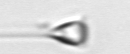
\includegraphics[height=1.6cm]{s1}}%
  \hspace{2em}%
  \subcaptionbox{}
      {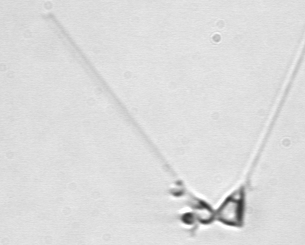
\includegraphics[height=2.5cm]{s2}}
  \hspace{2em}%
  \subcaptionbox{}
      {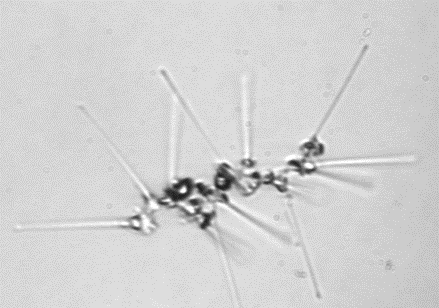
\includegraphics[height=2.5cm]{s3}}
  \caption{来自相同种类中的浮游生物,却表现出不相似的外形,即类内差异性}
\end{figure}

\begin{figure}[H]
  \centering%
  \subcaptionbox{} %标题的长度,超过则会换行,如下一个小图。
    {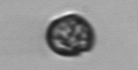
\includegraphics[height=1.8cm]{v1}}%
  \hspace{2em}%
  \subcaptionbox{}
      {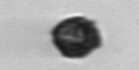
\includegraphics[height=1.8cm]{v2}}
  \hspace{2em}%
  \subcaptionbox{}
      {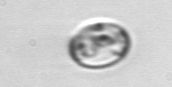
\includegraphics[height=1.8cm]{v3}}
  \caption{来自不同种类的浮游生物,却表现出相似的外形特点,即类间相似性}
\end{figure}


考虑到以上描述的浮游生物图像特点,使浮游生物图像的分类成为处于自然图像分类与细粒度分类之间的一种分类问题,因此依照目前传统的分类方法,即使用人工提取的特征(SIFT,HOG,LBP等)以及多种传统的分类器(NN,SVM,RF,DT等),很难有效地解决浮游生物图像分类问题。因此,在设计与实现浮游生物图像分类方法时,需要考虑浮游生物图像的特点,保证这些问题有效的解决。%但是由于浮游生物图像所存在的特殊性,正常适用于自然图像的特征提取方法,在提取浮游生物图像的特征方面,所取得的效果比较一般;而细粒度图像分类方法根据局部细节信息的判断方法,往往会忽略某些重要的全局特征信息,因此这中方法也不适用于浮游生物图像的分类。

%对于人类来说,首先往往是根据物体的形状进行区分的。但是由于之前我们已经讨论过浮游生物存在类间相似性与类内差异性,所以单纯根据浮游生物的外形形状进行类别的判断是不可靠的。在这种情况下,我们又可以根据浮游生物的纹理特征进行区分,即浮游生物的内部特征。对不同种类的浮游生物而言,其纹理总是不相同。对于同一种浮游生物种类而言,尽管这些浮游生物的形状可能是不相同的,但是纹理总是相似的。所以形状和纹理在浮游生物分类中起着非常重要的作用,为了更准确地对浮游生物图像进行分类,我们应该同时考虑形状特征和纹理特征。因此,在这里我们将原始图像转换为全局特征图像和局部特征图像,分别用来表示形状和纹理特征。随后通过将这些特征图像在卷积神经网络中训练以及混合,提高浮游生物图像的分类准确率。


%%%%%%%%%%%%%%%%%%%%%%%%%%%%%%%%%%%%%%%%%%%%%%%%%%%%%%%%%%%%%%%%%%%%%%%%%%%%%%%%%%%%%%%%%%%%%%%%%%%%%%%%%%%%%%%%%%
\section{多特征卷积神经网络模型}

相比较与传统的人工设计的特征提取和分类器方法,深度学习中的卷积神经网络是基于大量的图像数据以及具有强大学习能力的网络,通过巨大的计算量来获取更抽象和更高维度的信息,目前在图像分类与物体检测方面都取得了非常优异的成果。因此,在这里使用卷积神经网络的学习能力,来解决浮游生物图像分类问题。但是直接使用经典卷积神经网络模型,可能会由于浮游生物图像本身的特点,无法使网络模型发挥良好效果,需要对卷积网络模型进行改进。

\begin{figure}[H]
\centering
\begin{minipage}[b]{0.45\linewidth} 
      \centering 
      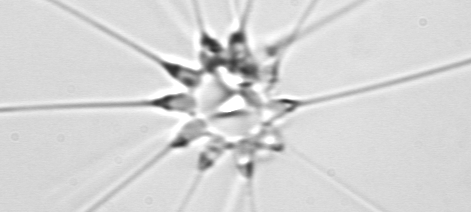
\includegraphics[width=0.75\linewidth]{shape1}
        \centerline{(a) }\medskip
\end{minipage}
  \begin{minipage}[b]{0.45\linewidth}
    \centering
    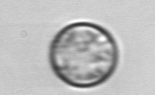
\includegraphics[width=0.65\linewidth]{shape2}
      \centerline{(b) }\medskip
  \end{minipage}
    \begin{minipage}[b]{0.45\linewidth}
    \centering
    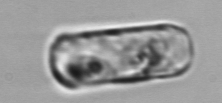
\includegraphics[width=0.75\linewidth]{shape3}
      \centerline{(c) }\medskip
  \end{minipage}
  \begin{minipage}[b]{0.45\linewidth}
    \centering
    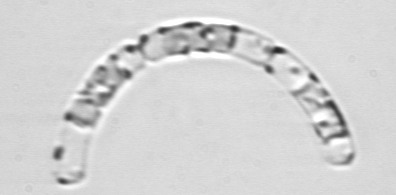
\includegraphics[width=0.75\linewidth]{shape4}
      \centerline{(d) }\medskip
  \end{minipage}
 \caption{不同种类的浮游生物图像}
\label{fig:plankton}
\end{figure}

为了有效地解决浮游生物图像分类问题,首先要对浮游生物图像的特点进行分析。对于人类识别物体,首先从物体的外观获取形状、大小、颜色等信息,通过对这些信息进行处理判断。如图~\ref{fig:plankton}所示,可以看出对于大多数浮游生物而言,不同种类的浮游生物在形状等形态特征方面仍然具有很大的差异,因此人类识别物体优先考虑外部形状,这种方法在浮游生物分类上仍可以使用。

但是如果只单纯从外部形状出发可能会造成很大问题。因为之前讨论过的类间相似性,即不同类别的浮游生物呈现相似的形状,如图~\ref{fig:similarity},如果考虑形状,那么很可能将不同种类的浮游生物归到同一个类别中;同时,由于类内相似性的存在,即相同类别的浮游生物呈现不同的形状,如图~\ref{fig:diff},那么很可能就会将相同类别的浮游生物划分为不同的类别。

\begin{figure}[H]
\centering
\begin{minipage}[]{0.42\linewidth} 
      \centering 
      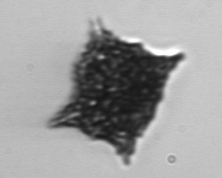
\includegraphics[height=3.2cm]{similarity1}
        \centerline{(a) }\medskip
\end{minipage}
  \begin{minipage}[]{0.42\linewidth}
    \centering
    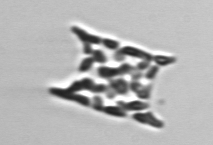
\includegraphics[height=3.1cm]{similarity2}
      \centerline{(b) }\medskip
  \end{minipage}
 \caption{两个不同种类的浮游生物图像,形状相似}
\label{fig:similarity}
\end{figure}

\begin{figure}[H]
\centering
\begin{minipage}[]{0.42\linewidth} 
      \centering 
      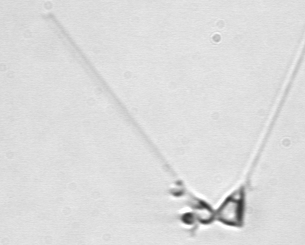
\includegraphics[height=3.2cm]{diff1}
        \centerline{(a) }\medskip
\end{minipage}
  \begin{minipage}[]{0.42\linewidth}
    \centering
    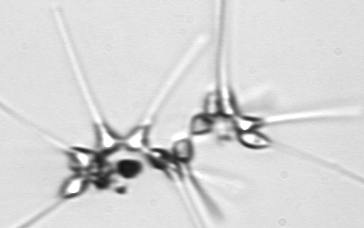
\includegraphics[height=3.1cm]{diff2}
      \centerline{(b) }\medskip
  \end{minipage}
 \caption{两个相同种类的浮游生物图像,形状不同}
\label{fig:diff}
\end{figure}

通过对浮游生物图像的不断研究,随后又发现了浮游生物内部的纹理具有很强的区分性。对于不同的浮游生物,内部纹理往往是不同的,如图~\ref{fig:texture1};而对于相同的浮游生物而言,纹理基本是相同的,如图~\ref{fig:texture2}。因此, 对于实现浮游生物图像分类,除了依靠形状信息外,纹理信息也是区分浮游生物的另一个重要特征。

\begin{figure}[H]
\centering
\begin{minipage}[]{0.45\linewidth} 
      \centering 
      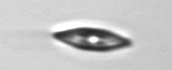
\includegraphics[height=2cm]{1}
        \centerline{(a) }\medskip
\end{minipage}
  \begin{minipage}[]{0.45\linewidth}
    \centering
    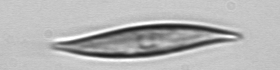
\includegraphics[height=1.7cm]{2}
      \centerline{(b) }\medskip
  \end{minipage}
 \caption{两个不同种类的浮游生物图像,纹理不同}
\label{fig:texture1}
\end{figure}

\begin{figure}[H]
\centering
\begin{minipage}[]{0.3\linewidth} 
      \centering 
      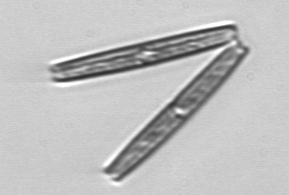
\includegraphics[height=2.5cm]{3}
        \centerline{(a) }\medskip
\end{minipage}
  \begin{minipage}[]{0.3\linewidth}
    \centering
    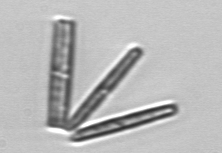
\includegraphics[height=2.5cm]{4}
      \centerline{(b) }\medskip
  \end{minipage}
  \begin{minipage}[]{0.3\linewidth}
    \centering
    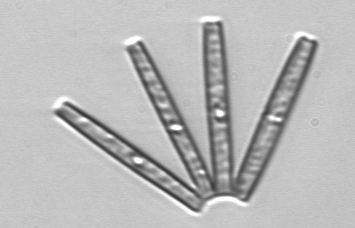
\includegraphics[height=2.5cm]{5}
      \centerline{(c) }\medskip
  \end{minipage}
  \caption{三个相同种类的浮游生物图像,纹理相同}
\label{fig:texture2}
\end{figure}

考虑到浮游生物图像所存在的类间相似性和类内差异性问题,可以结合形状信息和纹理信息,对浮游生物图像进行区分,但是在提取转换形状和纹理时,可能会造成浮游生物图像中部分重要信息的缺失,并且形状信息和纹理信息的侧重点不同,很难完美地进行结合,所以仍然需要对原始图像进行处理,提取所有信息。综合考虑以上因素,本论文提出了一种基于多特征卷积神经网络的浮游生物图像分类方法。

在生物形态学的角度,浮游生物图像中的形状信息和纹理信息是分析和处理浮游生物图像的关键信息;在计算机视觉的角度,可以将浮游生物图像的所有信息、形状信息和纹理信息转换为图像的原始特征、全局特征和局部特征。因此,在本网络模型中使用了三种不同的特征提取方法来描述浮游生物图像的特征,即原始特征、全局特征和局部特征,分别对应了图像中浮游生物的所有信息、形状信息和纹理信息。通过将这三种特征图像在模型中三个独立的卷积神经子网络中分别训练,不同子网络之间相互独立,使这些子网络只注重全部信息、形状信息和纹理信息这些具体特征的提取转换,而不用注重其他信息。在模型的最后部分是全连接层,通过对全连接层的交叉处理,保证不同特征的充分融合,对最终结果进行决策输出。

本论文所提出的多特征卷积神经网络模型结构如图~\ref{fig:architecture}所示。本网络模型是由三个卷积神经子网络组成,将这些子网络从左至右分别标记为网络A,网络B和网络C,从训练时间、网络大小以及网络性能等方面考虑,选择AlexNet作为基础子网络,不过不包括全连接层部分。本网络模型的1-5层为卷积层,6-8层为全连接层。

\begin{figure}[H] % use float package if you want it here
  \centering
  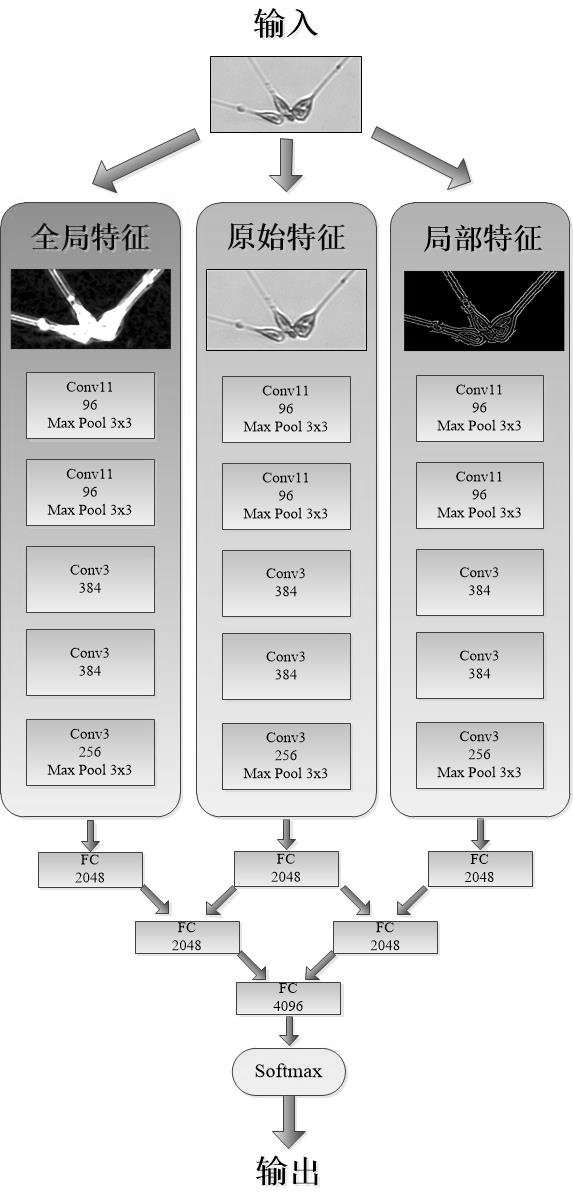
\includegraphics[height=17cm]{architecture}
  \caption{浮游生物图像分类的多特征卷积神经网络模型}
  \label{fig:architecture}
\end{figure}

如图~\ref{fig:architecture}所示,子网络A的第一个包含conv的方框表示卷积层,conv11表示卷积核的大小为11x11,96表示卷积核数目为96,Max pooling表示使用最大值池化,池化范围为3x3的像素块。同理,子网络A的最后一个包含conv的方框也表示卷积层,conv3表示卷积核的大小为3x3,384表示卷积核数目为384,Max pooling表示使用最大值池化,池化范围为3x3的像素块。第6层以后包含FC的方框表示全连接层,其中2048表示全连接层中神经元的个数。子网络A用来训练全局特征图像,子网络B用来训练原始图像,子网络C用来训练局部特征图像。其中,用来训练子网络A和C的全局特征图像和局部特征图像,输入图像在输入层经过数字图像处理和计算机视觉方法转换得到的。由于原始图像和全局特征图像以及局部特征图像之间有相同的尺寸,因此保证了各个网络的特征映射之间具有融合的可能性。在卷积层之后,本模型使用了倒金字塔形状的全连接结构,称之为交叉全连接层。考虑到在全局特征和局部特征之间具有巨大的差异,必须采取有效特殊的全连接结构实现特征融合,消除特征间的间隔。这里的交叉全连接层将两个子网络卷积之后的结果进行两两结合(全局特征与原始特征,原始特征与局部特征),最后将剩余两个结果进行融合,即通过原始图像所得到的内积作为连接局部特征和全局特征的桥梁。尽管该模型有三个输入数据,但是在网络处理和融合后只有一个输出,因此在训练过程的反向传播中,三个子网络共享同一个标签以及损失函数,保证了网络能够得到正常的训练。


%%%%%%%%%%%%%%%%%%%%%%%%%%%%%%%%%%%%%%%%%%%%%%%%%%%%%%%%%%%%%%%%%%%%%%%%%%%%%%%%%%%%%%%%%%%%%%%%%%%%%%%%%%%%%%%%%%%
\section{特征提取和特征融合}

\subsection{原始特征}
对于原始特征,我们需要采取基本的预处理:镜像映射、调整尺度、随机裁剪和减均值处理。图~\ref{fig:origin:a}表示输入到卷积神经网络模型的原始图像,图~\ref{fig:origin:b}表示原始图像经过调整尺度后的形式,蓝色方框代表随机裁剪后的区域。

\begin{figure}[H]
  \centering%
  \subcaptionbox{\label{fig:origin:a}} %标题的长度,超过则会换行,如下一个小图。
    {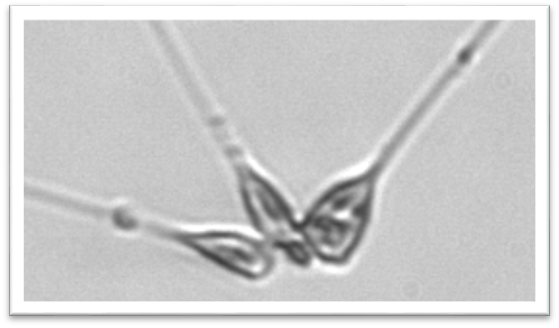
\includegraphics[height=3cm]{o}}%
  \hspace{4em}%
  \subcaptionbox{\label{fig:origin:b}}
      {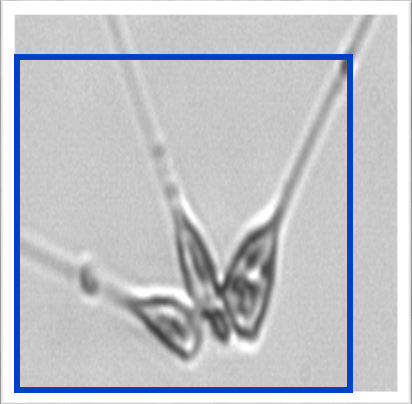
\includegraphics[height=3.5cm]{oa}}
  \caption{原始图像和经过预处理后的结果}
  \label{fig:origin}
\end{figure}

对于原始特征的预处理方法:
\begin{itemize}
\item 镜像映射:深度学习由于样本数据、网络模型以及训练方法的限制,经常会造成网络的过拟合。而最简单,也是最常用的方法是通过扩大数据集图像数量的方法来降低过拟合。镜像映射就是一种数据增强方法,通过在垂直方向上的映射,拓展样本数据的多样性。
\item 调整尺度:由于数据集中的图像大小经常不一致,而卷积神经网络对所有图像进行统一处理,因此在输入的时候,需要将图像进行尺度的调整。这里将所有图像的大小调整为256x256的形式,保证了所有输入图像尺度的统一,以及正常的训练。
\item 随机裁剪:图像中有许多信息是冗余的,而通过对输入图像的随机裁剪可以降低数据的维度,减少网络的计算量。另一方面,经过随机裁剪后的图像,一定程度增加了数据的随机性,可以降低过拟合现象。经过剪裁后图像的大小为224x224。
\item 减均值处理:根据所有输入图像计算出相应的均值图像,将每张图像的像素值进行减均值处理,是一种归一化方法,可以保证网络的有效训练,可以加快训练速度。另外,经过减均值处理,可以一定程度地提升准确率。
\end{itemize}



\subsection{全局特征}

由于网络模型中的全局特征表示了浮游生物的形状信息,而浮游生物的角毛和轮廓等形态特点都被视为是重要的形状信息\cite{zheng2014automatic},这些形态特点也是用来区分浮游生物种类的重要依据。所以,根据形状进行浮游生物类别的判断,是最直观也是最常用的方法。

但是想要提取出完整的浮游生物形状却不是容易的事情。由于浮游生物的形状较为复杂,细长的角毛、透明的细胞外膜、内部明显的细胞等因素,造成了浮游生物在外观形状上呈现多样化趋势;同时,因为浮游生物的角毛或细胞膜都为透明的,与背景十分相似,需要仔细观察才能够辨别出来。基于以上问题,使得传统的轮廓提取和图像分割的方法在提取浮游生物的形状信息时,都没有取得很好的效果。

因为形状信息主要注重浮游生物的外部轮廓,而不必关注内部纹理与图像背景。因此,如果能够突出浮游生物的形状轮廓,使其与背景产生强烈反差,即可有效提取出形状信息。在这里,本论文提出了一种图像处理的方法来解决这个问题,使图像中浮游生物的形状相比较于其它特征显得更明显与突出。
\begin{enumerate}
\item 首先,使用双边滤波器\cite{tomasi1998bilateral}消除浮游生物图像中的部分噪声,使图像中的浮游生物形状更加平滑。
\item 其次,使用基于Sobel算子优化的Scharr算子\cite{scharr2000optimal}将原始浮游生物图像转换为同时包含形状与纹理的图片形式。
\item 随后,为了使全局形状特征更加明显突出,由于浮游生物整体亮度较大,而背景颜色较深,因此使用对比度增强方法,使形状更加明显,移除内部特征。
\item 最后,经过对比度增强后的图像,可认为是充分表达形状信息的全局特征图像。
\end{enumerate}

\begin{figure}[H]
\centering
\begin{minipage}[]{0.3\linewidth} 
      \centering 
      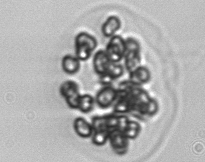
\includegraphics[height=2.5cm]{g1}
        \centerline{(a) }\medskip
\end{minipage}
  \begin{minipage}[]{0.3\linewidth}
    \centering
    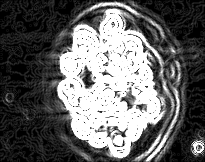
\includegraphics[height=2.5cm]{g2}
      \centerline{(b) }\medskip
  \end{minipage}
  \begin{minipage}[]{0.3\linewidth}
    \centering
    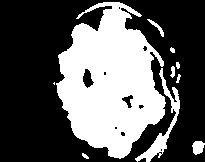
\includegraphics[height=2.5cm]{g3}
      \centerline{(c) }\medskip
  \end{minipage}
\begin{minipage}[]{0.3\linewidth} 
      \centering 
      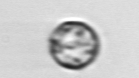
\includegraphics[height=2.2cm]{g4}
        \centerline{(d) }\medskip
\end{minipage}
  \begin{minipage}[]{0.3\linewidth}
    \centering
    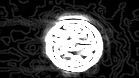
\includegraphics[height=2.2cm]{g5}
      \centerline{(e) }\medskip
  \end{minipage}
  \begin{minipage}[]{0.3\linewidth}
    \centering
    
\includegraphics[height=2.2cm]{g6}
      \centerline{(f) }\medskip
  \end{minipage}
  \caption{原始浮游生物图像,使用图像处理方法和图像分割方法得到的结果}
\label{fig:shape}
\end{figure}

图4-10(a)表示原始浮游生物图像,图4-10(b)表示经过本论文方法提取的全局特征图像,图4-10(c)表示使用图像分割技术grabcut\cite{rother2004grabcut}取得的全局特征图像。仅从外观上而言,图4-10(b)外观形状更明显,而图4-10(c)有部分形状信息缺失。图4-10(e)和图4-10(f)表示当grabcut方法能够有效地转换全局特征图像时,本论文方法也可以取得相应的结果。另外,将这些全局特征图像在AlexNet中进行实验,实验结果也表明了使用本论文的图像处理方法转换的全局特征图像所训练的网络,最终的分类准确率优于其他方法的结果。

\subsection{局部特征}

因为只根据形状信息区分浮游生物图像,结果往往是不可靠的。为了更有效的对浮游生物图像分类,需要另一个特征对形状信息进行补充。而由上述介绍可知,纹理信息相对于形状信息,是浮游生物另外一个非常重要的特征。相同种类的浮游生物,内部纹理基本相同;不同种类的浮游生物,内部纹理基本不相似。因此,可以使用纹理信息作为区分浮游生物种类的另外一个重要特征。

Canny算法\cite{canny1986computational}是一个多阶层的边缘算法,可以用来检测图像中大范围的边缘。Canny算法的目标在于检测图像中的最优边缘,即尽可能多地标识出图像中的实际边缘。这里将内部纹理信息理解为局部特征,使用Canny算法对内部特征进行提取转换。Canny算法的步骤可归纳为:
\begin{enumerate}
\item 降噪:通过将高斯平滑模板对原始图像进行卷积运算,得到有轻微模糊的图像。
\item 寻找图像中的亮度梯度:图像中的边缘可能会指向不同方向,这里使用水平方向、垂直方向以及对角线方向的4个掩膜对原始图像进行卷积运算。随后标注出各个像素点中的最大像素值和所生成的边缘方向,即可得到图像中像素点的亮度梯度图和亮度梯度方向。
\item 在图像中跟踪边缘:使用滞后阈值(高阈值和低阈值)对图像中的重要边缘进行跟踪标记,避免将噪声像素标记为边缘。
\end{enumerate}

通过对Canny算法中可调整参数(高斯滤波器的大小和阈值的设置)的修改,使Canny算法有效地跟踪标记出浮游生物的内部纹理信息,提取出浮游生物的纹理信息。图~\ref{fig:texture}表示原始图像和经过Canny算法转换后的局部特征图像。图4-11(a)和图4-11(c)从外观形状上非常相似,但是经过Canny算法提取局部特征之后,从图4-11(c)和图4-11(d)可以看出其内部纹理不相同,根据这点可对浮游生物图像进行区分。

\begin{figure}[H]
\centering
\begin{minipage}[b]{0.45\linewidth} 
      \centering 
      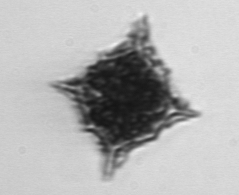
\includegraphics[width=0.75\linewidth]{l1}
        \centerline{(a) }\medskip
\end{minipage}
  \begin{minipage}[b]{0.45\linewidth}
    \centering
    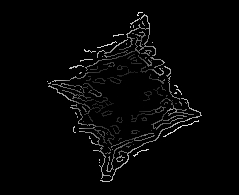
\includegraphics[width=0.75\linewidth]{l2}
      \centerline{(b) }\medskip
  \end{minipage}
    \begin{minipage}[b]{0.45\linewidth}
    \centering
    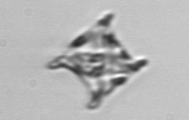
\includegraphics[width=0.75\linewidth]{l3}
      \centerline{(c) }\medskip
  \end{minipage}
  \begin{minipage}[b]{0.45\linewidth}
    \centering
    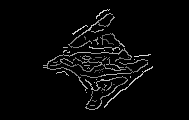
\includegraphics[width=0.75\linewidth]{l4}
      \centerline{(d) }\medskip
  \end{minipage}
 \caption{不同种类的浮游生物图像以及经过Canny算法转换的局部特征图像}
\label{fig:texture}
\end{figure}


%%%%%%%%%%%%%%%%%%%%%%%%%%%%%%%%%%%%%%%%%%%%%%%%%%%%%%%%%%%%%%%%%%%%%%%%%%%%%%%%
\subsection{交叉全连接层}

传统的网络融合方法主要是在全连接层计算后,直接对矢量相连进行融合。但是由于全局特征图像与局部特征图像是针对不同的视觉特点所提取的,那么在卷积神经网络训练时,最终所关注的重点信息将会有极大差别,如果直接融合可能反而会造成准确率的下降,因此需要一个更好的特征融合方式来提升分类结果。



如图4-12(a)表示普通的全连接融合,即只在最后一层进行矢量连接输出。但是由于在网络模型中,之前的子网络训练的特征具有较大差异,直接融合反而可能不会提升效果。原始图像中不仅具有全局特征,也包括局部特征。如果以原始特征为中介,进行融合以及继续训练,那么将能够更好地消除不同特征之间的间隙,实现特征的融合。因此本论文提出了以下的倒金字塔形式的全连接方式,即交叉全连接层,如图4-12(b)所示。交叉全连接层通过将不同特征进行两两结合,实现特征的融合以及重训练。

\begin{figure}[H]
\centering
\begin{minipage}[]{0.8\linewidth} 
      \centering 
      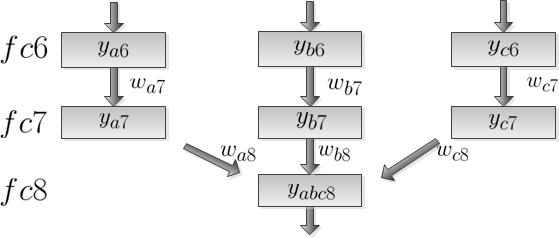
\includegraphics[height=4cm]{f1}
        \centerline{(a) }\medskip
\end{minipage}
  \begin{minipage}[]{0.8\linewidth}
    \centering
    \includegraphics[height=4cm]{f2}
      \centerline{(b) }\medskip
  \end{minipage}
 \caption{普通全连接层融合以及交叉全连接层}
%\label{fig:diff}
\end{figure}


FC6表示第六层为全连接层,同理,FC7和FC8同为全连接层。与之前所讨论的全连接层计算方式不同,从第6层到第7层的全连接训练的前向过程可以被归纳以下形式:
\begin{align}
y_{ab7m}=f(\sum_{i}^{2048} w_{71im}  y_{a6i} + \sum_{j}^{2048} w_{72jm}  y_{b6j} + b_{ab7}) \\
y_{bc7n}=f(\sum_{j}^{2048} w_{73jn}  y_{b6j} + \sum_{k}^{2048} w_{74kn}  y_{c6k} + b_{bc7}) 
\end{align}
$y_{ab7m}$表示第7层全连接层的左边层中第$m$个神经元的输出,$y_{bc7n}$表示第7层全连接层的右边层中的第$n$个神经元的输出。$w_{71im}$是第6层的第$i$个神经元到第7层的第$m$个神经元之间所对应的权值,$y_{a6i}$是子网络A中第6层的第$i$个神经元,$y_{b6j}$是子网络B中第6层的第$j$个神经元,$y_{c6k}$是子网络C中第$k$个神经元,$b_{ab7}$是第7层左边的偏置项,$b_{bc7}$是第7层右边的偏置项。相似的,$y_{abc8o}$也可以推导出。
\begin{equation}
y_{abc8o}=f(\sum_{m}^{4096} w_{81mo}  y_{ab7m} + \sum_{n}^{4096} w_{82no}  y_{bc7n} + b_{abc8})
\end{equation}

在反向传播时,误差传播相应的规则也必须遵从之前所提出的金字塔结构。特别地,在子网络B中,第6层的误差导数可以表示为如下形式:
\begin{equation}
\delta_{b6j}=f'(x_{b6j}) (\delta_{ab7m}  w_{72mj} + \delta_{bc7n}  w_{73nj})
\end{equation}
其中$\delta_{b6j}$是子网络B中第6层的第$j$个神经元的误差,$f'(x)$是激活函数的导数,请注意,只有子网络B会接收到从最后一层所传回的所有反向误差,而网络A和网络B将只接受从第8层传回的部分误差。

%%%%%%%%%%%%%%%%%%%%%%%%%%%%%%%%%%%%%%%%%%%%%%%%%%%%%%%%%%%%%%%%%%%%%
\section{具体步骤}

基于多特征融合卷积神经网络的浮游生物图像分类方法包括下列的具体步骤:
\begin{enumerate}
\item 采集清晰的浮游生物图像,构建大规模多类别的浮游生物图像数据集。该数据集中的浮游生物图像即为输入图像,在输入层对浮游生物输入图像进行预处理;

\item 通过对输入图像进行镜像映射、尺度调整、随机裁剪等预处理,得到原始特征图像


\item 通过对输入图像进行相应的数字图像处理,提取浮游生物的形状信息,得到全局特征图像:
\begin{enumerate}
\item 利用双边滤波法消除图像中的噪声,平滑图像中浮游生物的外部形状;
\item 利用Scharr算法对滤波后图像进行转换,得到中间结果图;
\item 使用增强对比度处理中间图,突出浮游生物的全局特征,忽略浮游生物的局部特征,得到的结果即为全局特征图像;
\end{enumerate}

\item 通过对输入图像使用计算机视觉中的Canny边缘检测算法,提取浮游生物内部的纹理信息,即浮游生物的局部特征,得到局部特征图像;

\item 将步骤2、步骤3及步骤4得到的原始特征图像、全局特征图像及局部特征图像输入到该多特征融合卷积神经网络模型中进行训练,最终得到优化后的多特征融合卷积神经网络模型:
\begin{enumerate}
\item 首先设置网络初始状态信息,包括迭代次数、学习率及初始化方式;
\item 对该多特征融合卷积神经网络模型进行前向和后向传播,使该多特征融合卷积神经网络模型以损失函数值为基础,根据权值梯度下降方向,对权值等参数进行更新和学习;
\item 随着不断迭代,损失函数值逐步下降,相应的准确率稳步上升;
\item 判断是否达到设置的迭代次数,如果是,则训练完毕,得到最终的多特征融合卷积神经网络模型;否则,继续跳转执行步骤6(b)继续训练;
\end{enumerate}

%\item 构建基于原始特征、全局特征及局部特征的多特征融合卷积神经网络模型,该多特征融合卷积神经网络包括三个相互独立的子网络,每个子网络分别训练原始特征图像、全局特征图像及局部特征图像,其中,该多特征融合卷积神经网络的1-5层为卷积层,6到8层为交叉全连接层;

\item 将待分类的浮游生物图像输入到最终的多特征融合卷积神经网络模型中,即可实现有效的浮游生物图像分类。 

\end{enumerate}

%进一步地,根据实际情况和需求,混合模型中的基础子网络可以使用AlexNet、GoogLeNet或者VGGNet中的任意一种基础卷积神经网络,混合模型最终的准确率根据所选择基础子网络的不同,会逐步提升,而相应地,模型训练时间代价也会逐步增长。

%%%%%%%%%%%%%%%%%%%%%%%%%%%%%%%%%%%%%%%%%%%%%%%%%%%%%%%%%%%%%%%%%%
\section{本章小结}
本章节主要介绍了本论文针对浮游生物图像分类问题,提出了基于多特征卷积神经网络结构模型具体的实现方法。由于浮游生物的种类庞大繁多,并且浮游生物存在类间相似性和类内差异性,使得普通的特征提取方法或机器学习都不能有效解决浮游生物图像分类问题。这里考虑到形状信息和纹理信息是辨别浮游生物种类重要的依据,另外原始图像也包含了重要的信息,因此将这三个特征图像都放在网络中进行训练与特征融合。多特征卷积神经网络模型是由三个卷积子网络组成,使用交叉全连接层实现特征的决策融合,是一个适用于浮游生物图像分类的深层卷积神经网络模型。









\chapter{多特征卷积神经网络的实验结果}

\section{实验基础}

由于第三章中的实验主要是自底向上地探究网络本身的关键因素,而且通过实验可知数据增强所取得的效果最好,但是数据增强只是单纯地增加图像数量,并没有对网络属性进行改进,没有本质上的提升,该网络也不能应用在其他数据集上。所以需要从另一个角度出发,从本质上提升网络性能,提升网络的学习能力和泛化能力,使网络能够应用到其他的浮游生物数据集上,具有更强的应用性。因此,在第四章的部分有经验指导性地对网络进行改进,自顶向下地对网络进行改进提升,在浮游生物分类的相关方法和知识的基础上,将浮游生物的特征融入到卷积神经网络中,通过构造更复杂和有效的网络结构在更大的数据集上取得更好的结果。

第三章的实验结果已经证明了基于深度学习的卷积神经网络在浮游生物数据集分类上的可行性,因此这里需要在浮游生物类别更多以及图像数量更多的数据集上进行实验,保证所提出的网络模型的有效性和实际可行性,因此选择之前介绍的浮游生物图像数据集中的的WHOI-Plankton数据集。但是对于该数据集而言,虽然其所提供的浮游生物图像无论从种类和数量上都是最多的,但是缺点也是非常明显的。因此,从WHOI-Plankton数据集中,随机挑选出每类的图像数量至少有1000张的30类浮游生物图像,然后在每类中随机挑选出1000张图像,用来保证数据集的平衡性以及最终结果的可靠性。将这些浮游生物图像随机分为两部分:训练集和测试集,训练集和测试集中的图像数量比例为4:1。训练集和测试集是随机采样所得。因此,本论文所构建的Plankton数据集有30类浮游生物总共3万张图像,该数据集中的图像如图~\ref{fig:dataimages}所示,该图中的每张小图就表示一种浮游生物,其中每类的浮游生物名字显示在表~\ref{table:name}中,小图是以行优先进行排列。在这个数据集训练多特征卷积神经网络,通过实验可以证明本文所提出的基于多特征卷积神经网络在浮游生物图像分类问题上的有效性以及可拓展性。

\begin{figure}[H] % use float package if you want it here
  \centering
  \includegraphics[height=8cm]{dataset}
  \caption{30类浮游生物的WHOI数据集中的浮游生物图像}
  \label{fig:dataimages}
\end{figure}

\begin{table}[H]\normalsize
\centering
\caption{30类浮游生物的WHOI数据集中的浮游生物类别名称}
\label{table:name}
\begin{tabular}{|c|c|c|c|}
\hline
序号 & 类别名字 & 序号 & 类别名字 \\
\hline
1 & Asterionellopsis & 16 & Guinardia\_flaccida \\ 
\hline
2 & Bad & 17 & Guinardia\_striata \\ 
\hline
3 & Chaetoceros & 18 & Heterocapsa\_triquetra \\
\hline
4 & Chaetoceros\_flagellate & 19 & Laboea\_strobila \\
\hline
5 & Ciliate\_mix & 20 & Leptocylindrus \\
\hline
6 & Corethron & 21 & Pennate \\
\hline
7 & Cylindrotheca & 22 & Phaeocystis \\
\hline
8 & Detritus & 23 & Pleurosigma \\
\hline
9 & Dictyocha & 24 & Prorocentrum \\
\hline
10 & Dino30 & 25 & Pseudonitzschia \\
\hline
11 & Dinobryon & 26 & Skeletonema \\
\hline
12 & Ditylum & 27 & Thalassionema \\
\hline
13 & Eucampia & 28 & Thalassiosira \\
\hline
14 & Flagellate\_sp3 & 29 & Thalassiosira\_dirty\\
\hline
15 & Guinardia\_delicatula & 30 & Tintinnid \\
\hline
\end{tabular}
\end{table}

本论文实验的软件环境是基于开源的深度学习框架Caffe(Convolutional Architecture for Fast Feature Embedding),硬件环境是基于四块英伟达的GTX Titan X显卡。在训练过程中,使用冲量为0.9和权值衰减系数为0.0005的随机梯度下降法。所有输出图像都会调整为256x256大小的尺寸,并且随机裁剪为227x227的大小;但是只有在原始特征图像的预处理使用减图像均值法,其他两种特征图像的预处理不需要。其他的参数初始化与AlexNet在ImageNet竞赛中使用的基本相同。

%%%%%%%%%%%%%%%%%%%%%%%%%%%%%%%%%%%%%%%%%%%%%%%%
\section{不同特征组合的分类实验结果}

为了验证多特征卷积神经网络在大数量的浮游生物图像分类上的有效性,以及该网络模型的合理性,这里同样设置多组实验对该模型进行分析与研究。多特征卷积神经网络模型同样使用 AlexNet 作为基础网络,考虑到AlexNet的训练时间、网络容量和分类准确率对于浮游生物图像分类都是比较合适的。为了考虑各种网络情况下,使用Plankton数据集上训练单网络、双网络和三网络的三组实验,在这些情况下分别对各个结果进行分析讨论:

\begin{enumerate}
\item 单特征网络AlexNet在数据集的训练

首先,只使用AlexNet分别对原始图像、全局特征图像、局部特征图像进行训练,可以得到单网络情况下AlexNet在Plankton数据集上的结果,如表~\ref{tab:single}。从表~\ref{tab:single}中可以看出,基于原始特征所训练的网络结果比基于全局特征图像和局部特征图像的网络结果都要好,可能是因为原始图像中所包含的信息更加丰富,其所训练的网络更加全面,而其他两种特征图像只包含其相对应的特征,因此所训练的网络比较片面。这里,将基于原始图像训练的AlexNet所对应的准确率94.75\%作为基础准确率,后续所有实验结果都是与该结果进行比较判断的。


\begin{table}[H]
\centering
\caption{单特征卷积神经网络在30类浮游生物图像数据上的结果}
\label{tab:single}
\begin{tabular}{|c|c|}%{|p{7cm}|p{1.8cm}<{\centering}|}
\hline
\centering{网络模型} & 准确率 \\
\hline
基于原始图像训练的AlexNet & 94.75\% \\ 
\hline
基于全局特征图像训练的AlexNet  & 94.06\% \\ 
\hline
基于局部特征图像训练的AlexNet  & 93.09\% \\
\hline
\end{tabular}
\end{table}

\item 双特征网络AlexNet在数据集的训练

因为特征融合的方法可以提升准确率,而在之前方法介绍了本方法是从多个维度对网络进行训练,因此尝试将两种不同的特征图像进行融合训练,判断网络结果最终是否得到提升。表~\ref{tab:double}表示了两种不同特征图像在Plankton数据集上的训练结果,经过原始图像信息的融合,全局特征图像和局部特征图像的训练结果都得到了提升,可能是由于原始图像信息丰富,对其余两种特征图像的信息进行了补充。而全局特征图像和全局特征图像由于之前讨论的,特征之间存在差异,较难很好地融合,因此结果几乎保持一致,没有明显提升。这里双网络的融合,是在全连接层进行矢量相连融合完成的。

\begin{table}[H]
\centering
\caption{双特征卷积神经网络在30类浮游生物图像数据上的结果}
\label{tab:double}
\begin{tabular}{|c|c|}%{|p{7cm}|p{1.8cm}<{\centering}|}
\hline
\centering{网络模型} & 准确率 \\
\hline
基于原始图像和全局特征图像训练的两个AlexNet & 95.32\% \\ 
\hline
基于原始图像和局部特征图像训练的两个AlexNet  & 94.50\% \\ 
\hline
基于全局特征图像和局部特征图像训练的两个AlexNet  & 93.33\% \\
\hline
\end{tabular}
\end{table}

\item 三特征网络AlexNet在数据集训练

对于三种特征共同训练的融合网络模型,在全连接部分可以使用直接相连的方法进行融合,但是由于不同特征之间所存在的差异,直接融合可能不会产生很好的结果。而且在全连接层中不同神经元连接数量也会有一定影响。表~\ref{tab:triple}表示三种特征训练的融合网络模型,但是没有使用交叉全连接层,而是使用最直接的全连接矢量相连的方式进行组合;另外,该表中也表示了在交叉全连接层使用不同的全连接神经元数量的影响。表~\ref{tab:triple}的结果说明了使用三种特征的网络模型相比于单特征网络模型和双特征融合网络模型,在结果上能有一定的提升。

\begin{table}[H]
\centering
\caption{全连接层设置不同,三特征融合卷积神经网络在30类浮游生物图像数据上的结果}
\label{tab:triple}
\begin{tabular}{|p{10cm}|p{1.8cm}<{\centering}|}
\hline
\centering{网络模型} & 准确率 \\
\hline
基于原始图像、全局特征图像和局部特征图像训练的三个AlexNet融合模型,没有交叉全连接层 &  95.67\% \\ 
\hline
基于原始图像、全局特征图像和局部特征图像训练的三个AlexNet融合模型,使用交叉全连接层,全连接层为4096个神经元  & 95.78\% \\ 
\hline
\end{tabular}
\end{table}


\item 基于AlexNet的多特征网络在数据集上的训练结果

本论文提出了使用原始图像、全局特征图像和局部特征图像相互融合的多特征卷积神经网络模型,在全连接层部分使用交叉全连接进行特征融合。表~\ref{tab:final}说明了使用交叉全连接的多特征融合的卷积神经网络在Plankton数据集上的实验结果。根据表~\ref{tab:triple}和表~\ref{tab:final}实验结果的比较,说明了使用交叉全连接层,可以提升准确率;另外,较少的全连接神经元,可以降低训练时间和过拟合现象,保证训练的有效性。

\begin{table}[H]
\centering
\caption{本论文所提出的多特征卷积神经网络在30类浮游生物图像数据上的结果}
\label{tab:final}
\begin{tabular}{|p{10cm}|p{1.8cm}<{\centering}|}
\hline
\centering{网络模型} & 准确率 \\
\hline
基于原始图像、全局特征图像和局部特征图像训练的三个AlexNet融合模型,使用交叉全连接层  & 95.83\% \\ 
\hline
\end{tabular}
\end{table}


\end{enumerate}

\section{网络拓展性的分类实验结果}
为了验证该多特征卷积神经网络的拓展性和实用性,这里将基础网络AlexNet替换为网络性能更好的GoogLeNet,继续进行实验。表~\ref{tab:google}表示了单特征GoogLeNet网络模型和多特征GoogLeNet网络模型在Plankton数据集上的训练结果。从表~\ref{tab:google}可知,通过网络性能更佳的GoogLeNet,相比较于AlexNet,在单网络模型上的准确率结果也有轻微提升。而对于多特征GoogLeNet网络模型在基于原始图像训练所得到的基础准确率95.2\%,也有一定程度的提升,说明了本方法的有效性。另外,由于GoogLeNet网络最后没有全连接层的存在,因此无法实现交叉全连接层。但是之前的实验已经说明了交叉全连接层的可靠性,如果这里使用交叉全连接层,最终分类准确率仍然可能还能再次提升。

\begin{table}[H]
\centering
\caption{单特征GoogLeNet网络模型和多特征GoogLeNet网络模型在30类浮游生物图像数据上的结果}
\label{tab:google}
\begin{tabular}{|c|c|}%{|p{7cm}|p{1.8cm}<{\centering}|}
\hline
\centering{网络模型} & 准确率 \\
\hline
基于原始图像训练的GoogLeNet & 95.2\% \\ 
\hline
基于全局特征图像训练的GoogLeNet  & 93.4\% \\ 
\hline
基于局部特征图像训练的GoogLeNet  & 93.2\% \\
\hline
基于三种特征图像训练的GoogLeNet  & 96.2\% \\
\hline
\end{tabular}
\end{table}

另外,为了保证实验结果的准确性,消除不确定因素等干扰,本章的实验结果已通过5次的随机交叉验证,最终的误差保证在0.1\%以内。

%%%%%%%%%%%%%%%%%%%%%%%%%%%%%%%%%%%%%%%%%%%%%%%%%%%%%%%%%%%%%%%%%%%%%
\section{本章小结}

本章节主要讨论了多特征卷积神经网络所使用的浮游生物数据集、以及多特征卷积网络模型在该浮游生物图像数据集上的分类实验结果。为了保证实验结果的合理性,本章节没有使用伍兹霍尔海洋研究所公布的WHOI-Plankton数据集,而是根据该数据集的分布特征,构建较为合理的Plankton数据集。另外,通过多组实验的设置,说明了本论文所提出的多特征卷积神经网络结构的合理性与有效性,并且将基础子网络替换,表明了该多特征网络结构具有良好的拓展性和泛化性。



\chapter{总结与展望}

\section{总结}

浮游生物在海洋生物圈和全球生态系统中起着重要作用,是海洋生物链的最底层,保证海洋生物圈的稳定,并且维持着全球生态系统的平衡。因此,对浮游生物的相关研究吸引了越来越多的关注。浮游生物图像的自动识别是一项非常重要的技术,其中就包括了浮游生物的自动分类。

传统的图像分类方法,主要是通过人工特征提取和分类器设计所完成的。但是由于浮游生物图像的特点,传统的图像分类方法并不适用于浮游生物图像的自动分类。基于深度学习的卷积神经网络,适用于解决大规模、复杂、困难的图像分类问题,与传统图像分类方法相比,能够挖掘出更抽象、更高维度的特征,
识别准确率更高,能更有效地解决问题。


本论文讨论了深度学习的基础理论和研究了多特征卷积神经网络的融合模型,进行了相关的探索和实验,主要研究工作如下:

\begin{enumerate}
\item 分析浮游生物图像特点,总结出浮游生物图像中存在的类间相似性和类内差异性问题,即不同种类的浮游生物,形状可能相似,纹理基本不同;而相同种类的浮游生物,形状可能不同,纹理基本相同。随后提出了形状和纹理相结合的浮游生物图像分析方法。
\item 将深度学习技术应用在多类别的浮游生物分类问题上,探究卷积神经网络在浮游生物图像分类问题的可行性。从自底向上的角度出发,根据网络深度、卷积数量、数据增强等方面对网络结构进行分析和改进。实验结果验证了卷积神经网络在解决浮游生物图像分类问题的有效性。
\item 从生物形态学与计算机视觉的角度,将浮游生物图像进行不同形式的变换,提出了一种基于多特征卷积神经网络的浮游生物图像分类方法。该方法从全部特征、形状特征和纹理特征出发,在多特征卷积网络模型中进行独立转换、训练和融合。该模型在多个不同维度的深层卷积网络基础上,对浮游生物图像进行分析处理和特征融合,将得到更具体和更高维度的特征,提升了网络模型的学习和表达能力。实验结果表明了该方法可以提升准确率,有效地解决浮游生物分类问题。
\end{enumerate}


\section{展望}

本论文提出了一种基于多特征卷积神经网络模型用于解决浮游生物图像分类问题,尽管该方法在实验中取得了较好的结果,但是仍然存在着不足之处需要在将来的工作继续改进:

\begin{enumerate}
\item 目前该基于多特征卷积神经网络的浮游生物图像分类方法是使用30类浮游生物图像数据集进行训练的,但是实际场景下,浮游生物种类可能超过100类以上,因此后续还需要收集更多数据对该方法进行训练测试,不断对其改进,保证该方法的实际可用性。
\item 该方法在提取全局特征图像的过程中,由于只是采用最简单的图像处理方法,所以在转换全局特征方面有所影响。在更高效的提取浮游生物形状信息的前提下,该方法可会得到更好的结果。
\item 由于该方法在训练过程中,需要对图像进行特征变换,而且网络模型有三个子网络,网络参数较多,另外全连接交叉也增加了全连接层的参数数量,一定程度上导致了训练时间增长和训练难度加大的问题。如果能减少训练时间,保证网络有效训练,那么就能提升网络模型的推广型和实用性。
\end{enumerate}


%%% 其它部分
%\backmatter

%% 本科生要这几个索引,研究生不要。选择性留下。
% 插图索引
%\listoffigures
% 表格索引
%\listoftables
% 公式索引
%\listofequations


%% 参考文献
% 注意:至少需要引用一篇参考文献,否则下面两行可能引起编译错误。
% 如果不需要参考文献,请将下面两行删除或注释掉。
\bibliographystyle{thuthesis}
\bibliography{ref/refs}


%% 附录
%\begin{appendix}
%\chapter{外文资料原文}
\label{cha:engorg}

\title{The title of the English paper}

\textbf{Abstract:} As one of the most widely used techniques in operations
research, \emph{ mathematical programming} is defined as a means of maximizing a
quantity known as \emph{bjective function}, subject to a set of constraints
represented by equations and inequalities. Some known subtopics of mathematical
programming are linear programming, nonlinear programming, multiobjective
programming, goal programming, dynamic programming, and multilevel
programming$^{[1]}$.

It is impossible to cover in a single chapter every concept of mathematical
programming. This chapter introduces only the basic concepts and techniques of
mathematical programming such that readers gain an understanding of them
throughout the book$^{[2,3]}$.


\section{Single-Objective Programming}
The general form of single-objective programming (SOP) is written
as follows,
\begin{equation}\tag*{(123)} % 如果附录中的公式不想让它出现在公式索引中,那就请
                             % 用 \tag*{xxxx}
\left\{\begin{array}{l}
\max \,\,f(x)\\[0.1 cm]
\mbox{subject to:} \\ [0.1 cm]
\qquad g_j(x)\le 0,\quad j=1,2,\cdots,p
\end{array}\right.
\end{equation}
which maximizes a real-valued function $f$ of
$x=(x_1,x_2,\cdots,x_n)$ subject to a set of constraints.

\newtheorem{mpdef}{Definition}[chapter]
\begin{mpdef}
In SOP, we call $x$ a decision vector, and
$x_1,x_2,\cdots,x_n$ decision variables. The function
$f$ is called the objective function. The set
\begin{equation}\tag*{(456)} % 这里同理,其它不再一一指定。
S=\left\{x\in\Re^n\bigm|g_j(x)\le 0,\,j=1,2,\cdots,p\right\}
\end{equation}
is called the feasible set. An element $x$ in $S$ is called a
feasible solution.
\end{mpdef}

\newtheorem{mpdefop}[mpdef]{Definition}
\begin{mpdefop}
A feasible solution $x^*$ is called the optimal
solution of SOP if and only if
\begin{equation}
f(x^*)\ge f(x)
\end{equation}
for any feasible solution $x$.
\end{mpdefop}

One of the outstanding contributions to mathematical programming was known as
the Kuhn-Tucker conditions\ref{eq:ktc}. In order to introduce them, let us give
some definitions. An inequality constraint $g_j(x)\le 0$ is said to be active at
a point $x^*$ if $g_j(x^*)=0$. A point $x^*$ satisfying $g_j(x^*)\le 0$ is said
to be regular if the gradient vectors $\nabla g_j(x)$ of all active constraints
are linearly independent.

Let $x^*$ be a regular point of the constraints of SOP and assume that all the
functions $f(x)$ and $g_j(x),j=1,2,\cdots,p$ are differentiable. If $x^*$ is a
local optimal solution, then there exist Lagrange multipliers
$\lambda_j,j=1,2,\cdots,p$ such that the following Kuhn-Tucker conditions hold,
\begin{equation}
\label{eq:ktc}
\left\{\begin{array}{l}
    \nabla f(x^*)-\sum\limits_{j=1}^p\lambda_j\nabla g_j(x^*)=0\\[0.3cm]
    \lambda_jg_j(x^*)=0,\quad j=1,2,\cdots,p\\[0.2cm]
    \lambda_j\ge 0,\quad j=1,2,\cdots,p.
\end{array}\right.
\end{equation}
If all the functions $f(x)$ and $g_j(x),j=1,2,\cdots,p$ are convex and
differentiable, and the point $x^*$ satisfies the Kuhn-Tucker conditions
(\ref{eq:ktc}), then it has been proved that the point $x^*$ is a global optimal
solution of SOP.

\subsection{Linear Programming}
\label{sec:lp}

If the functions $f(x),g_j(x),j=1,2,\cdots,p$ are all linear, then SOP is called
a {\em linear programming}.

The feasible set of linear is always convex. A point $x$ is called an extreme
point of convex set $S$ if $x\in S$ and $x$ cannot be expressed as a convex
combination of two points in $S$. It has been shown that the optimal solution to
linear programming corresponds to an extreme point of its feasible set provided
that the feasible set $S$ is bounded. This fact is the basis of the {\em simplex
  algorithm} which was developed by Dantzig as a very efficient method for
solving linear programming.
\begin{table}[ht]
\centering
  \centering
  \caption*{Table~1\hskip1em This is an example for manually numbered table, which
    would not appear in the list of tables}
  \label{tab:badtabular2}
  \begin{tabular}[c]{|m{1.5cm}|c|c|c|c|c|c|}\hline
    \multicolumn{2}{|c|}{Network Topology} & \# of nodes &
    \multicolumn{3}{c|}{\# of clients} & Server \\\hline
    GT-ITM & Waxman Transit-Stub & 600 &
    \multirow{2}{2em}{2\%}&
    \multirow{2}{2em}{10\%}&
    \multirow{2}{2em}{50\%}&
    \multirow{2}{1.2in}{Max. Connectivity}\\\cline{1-3}
    \multicolumn{2}{|c|}{Inet-2.1} & 6000 & & & &\\\hline
    \multirow{2}{1.5cm}{Xue} & Rui  & Ni &\multicolumn{4}{c|}{\multirow{2}*{\thuthesis}}\\\cline{2-3}
    & \multicolumn{2}{c|}{ABCDEF} &\multicolumn{4}{c|}{} \\\hline
\end{tabular}
\end{table}

Roughly speaking, the simplex algorithm examines only the extreme points of the
feasible set, rather than all feasible points. At first, the simplex algorithm
selects an extreme point as the initial point. The successive extreme point is
selected so as to improve the objective function value. The procedure is
repeated until no improvement in objective function value can be made. The last
extreme point is the optimal solution.

\subsection{Nonlinear Programming}

If at least one of the functions $f(x),g_j(x),j=1,2,\cdots,p$ is nonlinear, then
SOP is called a {\em nonlinear programming}.

A large number of classical optimization methods have been developed to treat
special-structural nonlinear programming based on the mathematical theory
concerned with analyzing the structure of problems.
\begin{figure}[h]
  \centering
  \includegraphics{thu-lib-logo}
  \caption*{Figure~1\quad This is an example for manually numbered figure,
    which would not appear in the list of figures}
  \label{tab:badfigure2}
\end{figure}

Now we consider a nonlinear programming which is confronted solely with
maximizing a real-valued function with domain $\Re^n$.  Whether derivatives are
available or not, the usual strategy is first to select a point in $\Re^n$ which
is thought to be the most likely place where the maximum exists. If there is no
information available on which to base such a selection, a point is chosen at
random. From this first point an attempt is made to construct a sequence of
points, each of which yields an improved objective function value over its
predecessor. The next point to be added to the sequence is chosen by analyzing
the behavior of the function at the previous points. This construction continues
until some termination criterion is met. Methods based upon this strategy are
called {\em ascent methods}, which can be classified as {\em direct methods},
{\em gradient methods}, and {\em Hessian methods} according to the information
about the behavior of objective function $f$. Direct methods require only that
the function can be evaluated at each point. Gradient methods require the
evaluation of first derivatives of $f$. Hessian methods require the evaluation
of second derivatives. In fact, there is no superior method for all
problems. The efficiency of a method is very much dependent upon the objective
function.

\subsection{Integer Programming}

{\em Integer programming} is a special mathematical programming in which all of
the variables are assumed to be only integer values. When there are not only
integer variables but also conventional continuous variables, we call it {\em
  mixed integer programming}. If all the variables are assumed either 0 or 1,
then the problem is termed a {\em zero-one programming}. Although integer
programming can be solved by an {\em exhaustive enumeration} theoretically, it
is impractical to solve realistically sized integer programming problems. The
most successful algorithm so far found to solve integer programming is called
the {\em branch-and-bound enumeration} developed by Balas (1965) and Dakin
(1965). The other technique to integer programming is the {\em cutting plane
  method} developed by Gomory (1959).

\hfill\textit{Uncertain Programming\/}\quad(\textsl{BaoDing Liu, 2006.2})

\section*{References}
\noindent{\itshape NOTE: These references are only for demonstration. They are
  not real citations in the original text.}

\begin{translationbib}
\item Donald E. Knuth. The \TeX book. Addison-Wesley, 1984. ISBN: 0-201-13448-9
\item Paul W. Abrahams, Karl Berry and Kathryn A. Hargreaves. \TeX\ for the
  Impatient. Addison-Wesley, 1990. ISBN: 0-201-51375-7
\item David Salomon. The advanced \TeX book.  New York : Springer, 1995. ISBN:0-387-94556-3
\end{translationbib}

\chapter{外文资料的调研阅读报告或书面翻译}

\title{英文资料的中文标题}

{\heiti 摘要:} 本章为外文资料翻译内容。如果有摘要可以直接写上来,这部分好像没有
明确的规定。

\section{单目标规划}
北冥有鱼,其名为鲲。鲲之大,不知其几千里也。化而为鸟,其名为鹏。鹏之背,不知其几
千里也。怒而飞,其翼若垂天之云。是鸟也,海运则将徙于南冥。南冥者,天池也。
\begin{equation}\tag*{(123)}
 p(y|\mathbf{x}) = \frac{p(\mathbf{x},y)}{p(\mathbf{x})}=
\frac{p(\mathbf{x}|y)p(y)}{p(\mathbf{x})}
\end{equation}

吾生也有涯,而知也无涯。以有涯随无涯,殆已!已而为知者,殆而已矣!为善无近名,为
恶无近刑,缘督以为经,可以保身,可以全生,可以养亲,可以尽年。

\subsection{线性规划}
庖丁为文惠君解牛,手之所触,肩之所倚,足之所履,膝之所倚,砉然响然,奏刀騞然,莫
不中音,合于桑林之舞,乃中经首之会。
\begin{table}[ht]
\centering
  \centering
  \caption*{表~1\hskip1em 这是手动编号但不出现在索引中的一个表格例子}
  \label{tab:badtabular3}
  \begin{tabular}[c]{|m{1.5cm}|c|c|c|c|c|c|}\hline
    \multicolumn{2}{|c|}{Network Topology} & \# of nodes &
    \multicolumn{3}{c|}{\# of clients} & Server \\\hline
    GT-ITM & Waxman Transit-Stub & 600 &
    \multirow{2}{2em}{2\%}&
    \multirow{2}{2em}{10\%}&
    \multirow{2}{2em}{50\%}&
    \multirow{2}{1.2in}{Max. Connectivity}\\\cline{1-3}
    \multicolumn{2}{|c|}{Inet-2.1} & 6000 & & & &\\\hline
    \multirow{2}{1.5cm}{Xue} & Rui  & Ni &\multicolumn{4}{c|}{\multirow{2}*{\thuthesis}}\\\cline{2-3}
    & \multicolumn{2}{c|}{ABCDEF} &\multicolumn{4}{c|}{} \\\hline
\end{tabular}
\end{table}

文惠君曰:“嘻,善哉!技盖至此乎?”庖丁释刀对曰:“臣之所好者道也,进乎技矣。始臣之
解牛之时,所见无非全牛者;三年之后,未尝见全牛也;方今之时,臣以神遇而不以目视,
官知止而神欲行。依乎天理,批大郤,导大窾,因其固然。技经肯綮之未尝,而况大坬乎!
良庖岁更刀,割也;族庖月更刀,折也;今臣之刀十九年矣,所解数千牛矣,而刀刃若新发
于硎。彼节者有间而刀刃者无厚,以无厚入有间,恢恢乎其于游刃必有余地矣。是以十九年
而刀刃若新发于硎。虽然,每至于族,吾见其难为,怵然为戒,视为止,行为迟,动刀甚微,
謋然已解,如土委地。提刀而立,为之而四顾,为之踌躇满志,善刀而藏之。”

文惠君曰:“善哉!吾闻庖丁之言,得养生焉。”


\subsection{非线性规划}
孔子与柳下季为友,柳下季之弟名曰盗跖。盗跖从卒九千人,横行天下,侵暴诸侯。穴室枢
户,驱人牛马,取人妇女。贪得忘亲,不顾父母兄弟,不祭先祖。所过之邑,大国守城,小
国入保,万民苦之。孔子谓柳下季曰:“夫为人父者,必能诏其子;为人兄者,必能教其弟。
若父不能诏其子,兄不能教其弟,则无贵父子兄弟之亲矣。今先生,世之才士也,弟为盗
跖,为天下害,而弗能教也,丘窃为先生羞之。丘请为先生往说之。”
\begin{figure}[h]
  \centering
  \includegraphics{thu-whole-logo}
  \caption*{图~1\hskip1em 这是手动编号但不出现索引中的图片的例子}
  \label{tab:badfigure3}
\end{figure}

柳下季曰:“先生言为人父者必能诏其子,为人兄者必能教其弟,若子不听父之诏,弟不受
兄之教,虽今先生之辩,将奈之何哉?且跖之为人也,心如涌泉,意如飘风,强足以距敌,
辩足以饰非。顺其心则喜,逆其心则怒,易辱人以言。先生必无往。”

孔子不听,颜回为驭,子贡为右,往见盗跖。

\subsection{整数规划}
盗跖乃方休卒徒大山之阳,脍人肝而餔之。孔子下车而前,见谒者曰:“鲁人孔丘,闻将军
高义,敬再拜谒者。”谒者入通。盗跖闻之大怒,目如明星,发上指冠,曰:“此夫鲁国之
巧伪人孔丘非邪?为我告之:尔作言造语,妄称文、武,冠枝木之冠,带死牛之胁,多辞缪
说,不耕而食,不织而衣,摇唇鼓舌,擅生是非,以迷天下之主,使天下学士不反其本,妄
作孝弟,而侥幸于封侯富贵者也。子之罪大极重,疾走归!不然,我将以子肝益昼餔之膳。”


\chapter{其它附录}
前面两个附录主要是给本科生做例子。其它附录的内容可以放到这里,当然如果你愿意,可
以把这部分也放到独立的文件中,然后将其 \cs{input} 到主文件中。

%\end{appendix}

%% 致谢
% 如果使用声明扫描页,将可选参数指定为扫描后的 PDF 文件名,例如:
% \begin{acknowledgement}[scan-statement.pdf]
\begin{acknowledgement}
时光匆匆如流水,转眼便又是毕业时节了,在我三年的硕士研究生生涯里,我所收获的不仅仅是愈加丰厚的知识,更重要的是思维方式和表达能力的转变与提升。我很庆幸在这三年我遇到了很多的良师益友,无论在学习上、生活上还是工作上,都给予了我无私的帮助和悉心的照顾,让我在一个温馨、有爱的环境中度过了我的三年研究生生活。

首先,我要感谢我的导师郑海永,这三年来给我最多教育和帮助的人!从我开始读研开始,郑老师一直对我严格要求,在他的指导下,我不仅树立了远大的学习目标,掌握了基本的研究方法,还明白了很多为人处世的道理。本论文从选题到最终完成,每一步都得到了郑老师的帮助和指点,在我迷茫时给予适时的鼓励,帮助我开拓研究思路,解决问题。感谢师母冯丽颖的关怀和教育,使我认识到自身的不足,从而努力提高自己,做一个坚强、会生活、懂生活的新时代女性。在此,谨向导师和师母表示崇高的敬意和衷心的感谢!

感谢实验室所有兄弟姐妹,没有你们的陪伴,我不会拥有这么美好、难忘的三年回忆。感谢我的实验室各位同学,在我的研究课题上给予了很多的支持和帮助,让我有了更大提高。

感谢我的家人,谢谢你们无私的付出,在我身后坚定地支持我、关心我、帮助我,有你们在,我更安心!

感谢国家自然科学基金项目“基于视觉注意结合生物形态特征的海洋浮游植物显微图像分析”(批准号:61301240)、国家自然科学基金项目“基于生物形态特征的中国海常见有害赤潮藻显微图像识别”(批准号:61271406)、中央高校基本科研业务费项目“海洋浮游动物原位探测与分析系统”(批准号:201562023)。

最后,感谢所有关心和帮助过我的人,祝愿你们幸福安康!
\end{acknowledgement}


%% 个人简历
\begin{resume}

  \resumeitem{个人简历}

  1991 年 08 月 21 日出生于 福建 省 霞浦 县。

  2010 年 9 月考入 河海大学 物联网工程 学院 通信工程 专业,2014 年 7 月本科毕业并获得 工学 学士学位。

  2014 年 9 月考入 中国海洋大学 电子 系攻读 硕士 学位至今。


  \resumeitem{发表的学术论文} % 发表的和录用的合在一起
     
  \begin{enumerate}[{[}1{]}]
  \item Dai J, Yu Z, Zheng H, Zheng B, Wang N. A Hybrid Convolutional Neural Network for Plankton Classification. ACCV 2016-Taipei, IEEE, 2017. (EI 收录)
  \item Dai J, Wang R, Zheng H, et al. ZooplanktoNet: Deep convolutional network for zooplankton classification. OCEANS 2016-Shanghai. IEEE, 2016. (EI 收录)
  \item Wang X, Dai J, Zhu Y, Zheng H and Qiao X. Spectral saliency via automatic adaptive amplitude spectrum analysis. Journal of Electronic Imaging, 2016. (SCI 收录)
  \end{enumerate}

  \resumeitem{在学期间参加的研究项目} % 有就写,没有就删除
  \begin{enumerate}
  \item 国家自然科学基金项目“基于视觉注意结合生物形态特征的海洋浮游植物显微图像分析”(批准号:61301240)
  \item 国家自然科学基金项目“基于生物形态特征的中国海常见有害赤潮藻显微图像识别”(批准号:61271406)
  \item 中央高校基本科研业务费项目“海洋浮游动物原位探测与分析系统”(批准号:201562023)
  \end{enumerate}
  


\end{resume}


%% 本科生进行格式审查是需要下面这个表格,答辩可能不需要。选择性留下。
% 综合论文训练记录表
%\includepdf[pages=-]{scan-record.pdf}
\end{document}
